% Author: David Paulino
% Date: 2023-03-03
% Description: LaTeX Template


\documentclass[12pt]{article}

% Document en français
\usepackage[french]{babel}

\usepackage[utf8]{inputenc}
\usepackage[T1]{fontenc}
\usepackage{graphicx}
\usepackage{amsmath}
\usepackage{amssymb}
\usepackage{amsthm}
\usepackage{amsfonts}
\usepackage{amscd}
\usepackage{amstext}

\usepackage{hyperref}
\usepackage{xcolor}
\usepackage{fancyhdr}
\usepackage{setspace}
\usepackage{float}
\usepackage{subfig}
\usepackage{caption}
\usepackage{listings}
\usepackage{tikz}
\usepackage{pgfplots}
\usepackage{pgfplotstable}
\usepackage{pgf}

% Add references in table of contents
\usepackage[nottoc]{tocbibind}

% Set author and place
\newcommand{\DP}{David Paulino}
\newcommand{\place}{Genève}
\newcommand{\fulltitle}{Analyse et optimisation de l'expected goal: application au machine learning}
\newcommand{\shorttitle}{Analyse et optimisation de l'expected goal}

% On retire l'indentation des paragraphes
\setlength{\parindent}{0pt}
% Augmentation de l'espacement entre les sauts de ligne
%\setlength{\parskip}{5pt} % Modifier la valeur selon vos besoins

% Title
\title{\fulltitle}
\author{\DP}
\date{\today}

% Header
\pagestyle{fancy}
\fancyhf{}
\renewcommand{\headrulewidth}{0pt}
\lhead{\DP}
\rhead{\shorttitle}

% Footers
\lfoot{Page \thepage}
\rfoot{\today}

% Document
\begin{document}

% Title page
\begin{titlepage}

    \begin{figure}[h]
        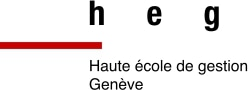
\includegraphics[width=0.3\textwidth]{img/logo_heg-ge.jpg}
    \end{figure}

    \vspace*{0.5cm}

    \begin{center}

        \begingroup \linespread{1,75} \selectfont
        {\Large \fulltitle}\\[0,75cm]
        \endgroup


        % Make a vertical space

        \vspace{1.5cm}

        \textsc{\large Travail de Bachelor HES réalisé en vue de \newline l’obtention du Bachelor par :}\\[0,50cm]

        \begingroup \linespread{1,5} \selectfont
        \textsc{\large \DP}\\[0,50cm]
        \endgroup


        \vspace{1cm}


        \textsc{\large Conseillers au travail de Bachelor : }

        \begingroup \linespread{1,5} \selectfont
        \textsc{\large Pr Alexandros KALOUSIS}\\[0.1cm]
        \textsc{\large Dr Nils SCHÄTTI}\\[1cm]
        \endgroup


        \begingroup \linespread{1,75} \selectfont
        \textsc{\large \place, le \today}\\[0,1cm]

        {\large Haute école de Gestion de Genève (HEG-GE)}\\[0,1cm]

        {\large Filière Informatique de gestion}\\[0,1cm]
        \endgroup



        \begin{figure}[h]
            \vspace{0.05cm}
            \hspace*{12cm}
\includegraphics[width=0.25\textwidth]{img/logo_hes-so.jpg}
        \end{figure}

    \end{center}



    \vfill
\end{titlepage}




\newpage

% Table of contents
\tableofcontents
\newpage

% Content
\section{Introduction}

% Citation avec Zotero et BibLaTeX
\subsection{Introduction à la problématique}
Lorsque les premiers sports sont apparus, l'information la plus importante était le score et le vainqueur de la confrontation.
Au fur et à mesure, plus d'informations sur les matchs sont venues s'ajoutées.
Le nombre de tirs dans un matchs par équipes, le nombre de passes, le nombre de tirs cadrés, la possession du ballon, le pourcentage de passes réussies, le nombre de passes décisives et d'autres sont venus s'ajouter aux statistiques dans le football.
Le pourcentage de réussite aux lancers francs, le nombre de rebonds, le nombre de passes décisives, le pourcentage de réussite aux tirs, le nombre de fautes, le nombre de minutes jouées, le pourcentage de réussite à 3 points et d'autres sont venus s'ajouter aux statistiques dans le basketball.
Ces statistiques sont également devenus personnelles à chacun des joueurs.
On peut également compter pour le baseball le nombre de fois qu'un joueur était au bâton, son nombre de double, de triples, son nombre de buts et bien d'autres.
\newline\newline
C'est d'ailleurs dans le baseball que l'on peut retrouver la première utilisation de statistiques avancées pour établir des stratégies.
En effet, au début des années 1970, le joueur des Baltimore Orioles a développé une analyse statistiques pour choisir le meilleur alignement possible pour son équipe de départ.
Cependant, il n'a pas pu l'utiliser à ce moment-là puisque le président de sa franchise n'avait pas confiance. C'est qu'à partir de 1984 où il fut le coach des New York Mets qu'il a pu mettre en place son analyse statistiques avancées pour établir le meilleur choix pour son équipe de départ. \cite{incPCMag1984}
Deux saisons plus tard, il remporte la Série mondiale 1986 \footnote{En MLB, la Série mondiale est la série finale qui permet de déterminer qui est l'équipe championne de la ligue.}. Les Mets étaient situés à la dernière place de leur conférence avant l'arrivée de Davey Johnson et son management orienté sur les statistiques.
\newline
Après cette réussite, les autres franchises de la MLB\footnote{Ligue majeure de baseball} ont également commencé à adopter l'analyse de statistiques dans le sport et cela a également été populaire dans les autres sports avec par exemple Daryl Morey qui a été le premier coach analyste statistiques recruté chez les Rockets de Houston en NBA en 2007. \cite{DarylMorey13year2020}
Les franchises de la NBA\footnote{Ligue nationale de basketball} ont par la suite également adopté une approche managériale statistique.
On constate alors que cette culture de la statistique dans le sport provient des États-Unis.
\newline
Il est désormais important d'amener l'arrivée des expected goals. L'une des premières études sur un modèle d'expected goals vient d'Alan Ryder qui a publié une étude sur la qualité des tirs effectuées dans des matchs de hockey. \cite{ryderIsolatingShotQuality2004}
Ce dernier a pu analyser les différentes circonstances lors d'un tir et développer un modèle qui prédit la probabilité d'un tir selon les circonstances de ce tir.
Dans le football, l'une des premieres études sur l'expected goal vient de Richard Pollard, Jake Ensum et Samuel Taylor qui ont analysé les facteurs qui influent la chance de marquer un but. \cite{pollardEstimatingProbabilityShot2004} La problématique de ce travail est donc de pouvoir analyser et optimiser l'expected goal.
\newline\newline
Il semble maintenant important de savoir ce qu'est l'expected goal. L'expected goal
\footnote{Très souvent réduit par xG} est une métrique qui permet de déterminer la probabilité qu'un tir soit transformé en but selon les données de ce tir \cite{XGExplainedFBrefa}.
Un tir qui a un xG de 0.4 a une probabilité de 40\% d'être transformé en but. Un tir avec un xG à 1 est la plus grande valeur possible et aurait donc 100\% de chance d'être transformé en but.
\footnote{Il est important d'indiquer qu'il est très rare qu'un xG d'un tir soit égal à 1 mais il va généralement s'en rapprocher fortement selon ses paramètres.} \cite{pettyWhatExpectedGoals2018a}
\newline\newline
Pour observer ce qu'est réellement un xG, nous allons l'observer avec l'emplacement des tirs sur le terrains.
Sur la figure \ref{fig:shotmap}, on peut observer un example d'emplacement de tirs et de leur xG.
\newline \newline
Par ailleurs, les xG se sont tellement développés que des métriques dérivées ont été créées. On peut par exemple citer le xA qui est l'expected assist. C'est une métrique qui permet de déterminer la probabilité qu'une passe soit transformée en passe décisive selon les données de cette passe. \cite{XGExplainedFBrefa}
Également, les xGA qui est les expected goals against. Cette métrique permet de déterminer la probabilité qu'un tir soit transformé en but selon les données de ce tir mais pour l'équipe adverse. \cite{pettyWhatExpectedGoals2018a}

Il y en a également d'autres comme les expected points qui sont les points qu'une équipe devrait avoir gagnés basé sur les données relatives aux xG. D'autres dérivées sont indiquées sur l'article de Pinnacle écrit par Luke Petty. \cite{pettyWhatExpectedGoals2018a}
\newline\newline
Maintenant que nous avons vu ce qu'est un xG et ces dérivées actuelles, il semble pertinent de décrire l'utilisation de cette métrique dans le football actuel.

\begin{figure}[htp]
    \centering
    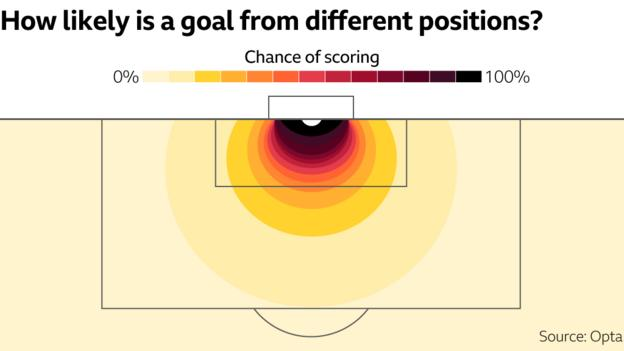
\includegraphics[width=0.8\textwidth]{img/SchemaXG.jpeg}

    \caption{Schéma qui montre les chances de buts selon les positions des tirs - Source : Opta}
    \label{fig:shotmap}
\end{figure}
\subsection{Intérêt de la problématique}
Cette problématique est très intéressante puisque c'est une donnée qui est dernièrement très populaire dans le monde du football. Elle donne plus d'informations sur le match que les autres statistiques d'un matchs (possession, nombre de passes, nombre de tirs cadrés, nombre de buts, etc.). Par exemple en ce qui concerne la possession, une équipe peut avoir la possession du ballon pendant 70\% du match mais ne pas marquer de buts, ni même être dangereuse avec le ballon. Le nombre de tirs cadrés, s'ils sont effectuées tous à l'extérieur de la surface de réparation, ne sont pas forcément dangereux. L'expected goal permet de donner une valeur à chaque tir et de déterminer si un tir a une chance d'être transformé en but.
\newline \newline
Certaines personnes utilisent cette métrique pour leurs paris sportifs. Ils observent la métrique lors des derniers matchs et la compare avec le score réel du match. Si la différence est grande, cela peut permettre de constater un manque de réalisme ou un sur-régime d'une des deux équipes. \cite{tennerelBienUtiliserExpected2022a}
\newline \newline
Les analystes de données des équipes utilisent cette donnée pour analyser les performances de leurs joueurs et de leurs équipes. Par exemple, la comparaison des xG et du nombre de buts marqués d'un joueur sur une période donnée peut permettre de déterminer la dangerosité et la capacité d'un buteur à terminer des actions. \cite{pettyWhatExpectedGoals2018a}
Les xG peuvent aussi être utilisés pour analyser les performances d'une équipe dans des situations bien précises. Une équipe qui possède un haut xG sur des contre-attaques montre qu'elle est très dangereuse sur ce type de situation. \cite{XGExplainedFBrefa}
L'une des choses les plus intéressante de cette métrique est qu'elle peut être utilisée pour analyser les forces et faiblesses des équipes. Par exemple, une équipe peut observer que ses xG sont très faibles lorsqu'elle tente des centres. Cela peut lui permettre de trouver son identité de jeu et de décider d'abandonner cette stratégie. Cette métrique est tout autant valable pour analyser les forces et faiblesses d'une équipe adverse. Dans la même situation, si une équipe vient à affronter l'équipe qui a dû mal à produire des xG sur des centres, elle peut décider de la forcer à jouer sur des centres en libérant de l'espace sur les côtés par exemple.
\newline \newline
Cette métrique est également utilisée pour aider les recruteurs à juger les performances de finition d'un joueur \cite{garratt-stanleyWhatExpectedGoals2022}. Nous avons vu précédemment qu'il existait des dérivées des xG comme les xA\footnote{Passes décisives attendues}. Les différentes dérivées peuvent permettre de juger les performances et qualités d'un joueur qui se trouve dans un poste bien précis. Par exemple, un milieu de terrain ou un défenseur peut être jugé sur ses xA et un attaquant sur ses xG.


\subsection{Questions que l'on souhaite répondre dans ce travail}
Il y a deux grandes questions à répondre dans ce travail.
\begin{itemize}
    \item Quels sont les paramètres qui influencent le plus l'expected goal ?
    \item Quel est le meilleur modèle pour prédire l'expected goal ?
\end{itemize}

Le but de ce travail est de comprendre quelles sont les variables qui influences le plus les xG.
Cela permettra de comprendre quelles sont les variables les plus importantes pour prédire les xG.
Grâce à cela, il est possible pour un analyste de données d'une équipe de football de savoir quelles sont les facteurs qui influencent le plus la qualité d'un tir.
Cela peut permettre de déterminer les forces et faiblesses d'une équipe et de savoir sur quels aspects travailler pour améliorer les performances de l'équipe.
\newline \newline
Le deuxième objectif de ce travail est de trouver le meilleur modèle pour prédire les xG.
En effet, le but sera d'avoir le modèle le plus performant et de comparer les différents modèles qui peuvent être utilisée pour établir cette métrique.
Il faut également veiller à ce que le modèle ne fasse pas de sur-apprentissage. Il est donc important de faire attention à la complexité du modèle et de trouver le meilleur compromis entre la complexité et la performance du modèle.

\newpage
\section{Plan du document}
Concernant le déroulement de ce travail, il y a plusieurs étapes.
Tout d'abord, il y a la recherche des travaux existants sur le sujet.
Parmi les travaux existants, je vais chercher à savoir quels datasets ont été utilisées ainsi que les résultats obtenus.
Cela me permettra de comparer mes résultats avec les résultats obtenus dans les autres travaux.
\newline \newline
La suite sera de trouver un dataset avec les informations nécessaires pour implémenter le modèle.
Une fois ce dataset trouvé, il va falloir le documenter. En effet, il est important de comprendre ce que chaque attribut représente.
L'étape suivante est également importante puisque le but sera de visualiser les données.
Cela permettra de voir si les données sont exploitables et si elles sont cohérentes.
Cela pourra également nous indiquer si des biais seront présents dans le modèle.
\newline \newline
Une fois que les données sont documentées et visualisées, il va falloir les préparer.
En effet, il pourrait y avoir des données manquantes mais qui sont disponibles après un traitement.
Il pourrait également y avoir des données qui ne sont pas exploitables et qui doivent être supprimées.
Par exemple, l'identifiant de la base de données d'un tir pourrait être supprimée car il n'appporte rien pour la prédiction de l'expected goal.
\newline \newline
Ensuite, on pourra commencer à implémenter le modèle et observer les facteurs qui influencent le plus sa prédiction du xG.
C'est également à ce moment-là qu'il faudra comparer les différents modèles pour voir lequel est le plus performant pour prédire les xG.
Il sera également intéressant de voir quelles variables peuvent être ajoutées au modèle pour améliorer sa précision.

\newpage
\section{Synthèse des travaux existants}
\label{sec:synthese}
Le premier travail repertorié sur les xG et la qualité d'un tir est celui de Richard Pollard, Jake Ensum et Samuel Taylor \cite{pollardEstimatingProbabilityShot2004}.
Dans ce travail datant de 2004, la seule information indiquée concernant le dataset est que les données proviennent de la Coupe du monde 1986 et de celle de 2002.
Le modèle a été implémenté en utilisant une régression logistique.
Le nombre de tirs répertoriées dans ce travail est de 1096.
La conclusion de ce travail est que les 3 facteurs les plus influents pour la prédiction des xG sont :
\begin{itemize}
    \item La distance entre le tireur et le but
    \item L'angle du but en fonction de la position du tir
    \item L'espace entre le tireur et le défenseur le plus proche
\end{itemize}
Le résultat final de l'analyse de la régression logistique de ce travail ressemble à cela.
\begin{table}[htp]
    \centering
    \begin{tabular}{|l|l|l|l|l|l|l|}
        \hline
        \textbf{Predictor} & \textbf{Coefficient} & \textbf{z} & \textbf{p} & \textbf{ratio} & \textbf{Lower} & \textbf{Upper} \\ \hline
        Constant           & 0.3771               & 1.20       & 0.229      &                &                &                \\ \hline
        Distance           & -0.1586              & -9.51      & 0.000      & 0.85           & 0.83           & 0.88           \\ \hline
        Angle              & -0.0222              & -3.81      & 0.000      & 0.98           & 0.97           & 0.99           \\ \hline
        Space              & 0.7991               & 3.22       & 0.001      & 2.22           & 1.37           & 3.62           \\ \hline
    \end{tabular}
    \caption{Résultat de la régression logistique du travail de Pollard, Ensum et Taylor}
\end{table}

Le deuxième travail est celui de Izzatul Umami, Deden Hardan Gutama et Heliza Rahmania Hatta \cite{umamiImplementingExpectedGoal2021}. 
Ce travail utilise les données de Wyscout des 5 championnats majeurs en Europe de la saison 2019-20. Ces derniers ont décidés de prendre comme données :
\begin{itemize}
    \item La distance
    \item L'angle
    \item Si le tir est un tir de la tête ou pas
\end{itemize}
Dans le dataset, 32000 tirs ont été utilisées pour la création du modèle.
Comme pour le travail précédent, la régression logistique a été utilisée.
Il est également indiqué qu'une séparation du dataset a été faite pour avoir des données d'entraînement et de tests.
Dans leurs tests du modèle, il est indiqué que le but est de faire de la classification pour de futures instances, il faut donc utiliser un seuil.
Suite à l'utilisation d'un seuil pour la classification, une matrice de confusion a été faite pour ensuite calculer la spécificité et la sensibilité du modèle.
Ce principe de sensibilité et spécificité permet de choisir la meilleure performance selon le contexte d'utilisation du modèle.
\begin{equation}
    Sensitivity = \frac{True Positive}{True Positive + False Negative}
\end{equation}
\begin{equation}
    Specificity = \frac{True Negative}{True Negative + False Positive}
\end{equation}
La sensibilité permet de voir la capacité du modèle à prédire correctement les tirs qui sont des buts.
De l'autre côté, la spécificité permet de voir la capacité du modèle à prédire correctement les tirs qui ne sont pas des buts.
Comme indiqué dans le travail de Umami, Gutama et Hatta, la spécificité est plus importante que la sensibilité selon le contexte.
Dans le cas où le modèle est utilisé pour prédire un cancer, nous allons chercher à avoir une meilleur sensibilité pour éviter de passer à côté d'un cancer. \cite{umamiImplementingExpectedGoal2021}
Cela leur permet de savoir comment choisir le seuil pour la classification.
En conclusion de leur travail, ils ont obtenu une sensibilité de 0.9671945701357466 et une spécificité de 0.19034406215316316 pour un seuil 0.02.
Ils indiquent finalement que le modèle de xG est plus performant si l'on prend la distance et l'angle en compte plutôt que de prendre uniquement la distance.
Un graphique ROC \footnote{Receiver Operating Characteristic} a été fait pour montrer la performance du modèle. Cela permet de comparer la sensibilité et la spécificité pour chaque seuil.
\newline\newline
Un autre travail qui fournit également du code est celui de David Sumpter \cite{sumpterFittingXGModel}. 
Le travail de ce dernier est de créer un modèle de xG en utilisant une régression logistique. 
Il utilise les données de Wyscout du championnat anglais de la saison 2017-18. 
Ce dernier explique étape par étape ce qui est effectué pour créer et améliorer son modèle.
Il y a également des pistes pour convertir les positions X et Y en distance et en angle.
Il commence par créer un modèle de xG en utilisant uniquement la distance. 
Par la suite, il le fait uniquement avec l'angle.
Ensuite, il utilise de multiples facteurs, comme la distance au carré ou encore l'angle multiplié par la position X du tir, pour créer son modèle et il produit un résumé de la régression logistique.

\begin{table}[htp]
    \centering
    \begin{tabular}{|l|l|l|l|l|l|l|}
    \hline
    \textbf{Predictor} & \textbf{coef} & \textbf{std err} & \textbf{z} & \textbf{P\textgreater{}|z|} & \textbf{{[}0.025} & \textbf{0.975{]}} \\ \hline
    Intercept          & -0.5103       & 0.887            & -0.576     & 0.565                       & -2.248            & 1.228             \\ \hline
    Angle              & -0.6338       & 0.319            & -1.989     & 0.047                       & -1.258            & -0.009            \\ \hline
    Distance           & 0.2798        & 0.118            & 2.381      & 0.017                       & 0.049             & 0.510             \\ \hline
    X                  & -0.1243       & 0.124            & -1.001     & 0.317                       & -0.368            & 0.119             \\ \hline
    C                  & 0.0300        & 0.040            & 0.750      & 0.454                       & -0.048            & 0.109             \\ \hline
    X2                 & -0.0014       & 0.001            & -1.422     & 0.155                       & -0.003            & 0.001             \\ \hline
    C2                 & -0.0041       & 0.003            & -1.398     & 0.162                       & -0.010            & 0.002             \\ \hline
    AX                 & 0.1251        & 0.118            & 1.063      & 0.288                       & -0.105            & 0.356             \\ \hline
    \end{tabular}
    \caption{Résumé de la régression logistique du modèle de xG de David Sumpter}
\end{table}
Il n'y a pas moyen de connaître les coefficients uniquement pour la distance et l'angle car aucun résumé n'est fait pour ces deux facteurs uniquement.
\newline\newline
Le dernier travail est fait par H.P.H Eggels. 
Le but est d'expliquer le résultat d'un match en utilisant les xG. 
Dans ce travail, il utilise un modèle de xG pour prédire le résultat d'un match.
Les données du travail proviennent de ORTEC, de Immotio et FIFA. En effet, son travail utilise trois datasets pour créer son modèle de xG. \cite{eggelsExpectedGoalsSoccer2016}.
Il y a eu un travail de "merging" des données pour avoir un dataset qui contient toutes les informations nécessaires pour créer le modèle. 
Cependant, les datasets peuvent avoir des problèmes entre eux lors du "merging". 
Par exemple, les noms des joueurs qui sont différents (majuscule, accent, encodage, surnom, etc.) a été un problème mais une solution a été trouvée.
\newline
Le dataset utilisé contient donc trois sources de données différentes.
\begin{table}[htp]
    \centering
    \begin{tabular}{lll}
    \hline
    \textbf{ORTEC}  & \textbf{FIFA}       & \textbf{Immotio}                  \\ \hline
    Context         & Player quality      & Number of attackers in line       \\
    Part of body    & Goal keeper quality & Number of defenders in line       \\
    Dist to goal    &                     & Distance nearest defender in line \\
    Angle to goal   &                     & Distance goal keeper              \\
    Originates from &                     &                                   \\
    Current score   &                     &                                   \\
    High            &                     &                                   \\ \hline
    \end{tabular}
    \caption{Sources de données utilisées par H.P.H Eggels}
\end{table}
\newpage
Parmi les modèles testés, ce travail utilise :
\begin{itemize}
    \item Un modèle de régression logistique
    \item Random Forest
    \item Un arbre de décision
    \item Ada-boost
\end{itemize}
Pour chacun de ces modèles, il y a une liste des différents paramètres qui vont être utilisés pour trouver le meilleur modèle.
Chacun des modèles a suivi une procédure avec un set d'entraînement, un set de validation et un set de test.
Le set de validation permet de trouver les meilleurs paramètres pour le modèle.
Le set de test permet de tester le modèle avec les paramètres trouvés et le comparer avec les autres modèles
Le modèle le plus performant parmi les quatres cités est le Random Forest avec une précision de 0.771.
Cependant, il n'est pas possible de connaître les meilleurs hyper paramètres pour chacun des modèles.
Ce travail donne tout de même de bonnes pistes pour l'ajout de nouvelle données pour améliorer le modèle de xG.


\subsection{Récapitulatif des travaux existants}
\begin{table}[htp]
    \centering
    \begin{tabular}{lll}
    \hline
    \textbf{Auteur(s)}                                                                                   & \textbf{Source de données}                                                                               & \textbf{Conclusion}                                                                                                                                          \\ \hline
    \begin{tabular}[c]{@{}l@{}}Richard Pollard\\ Jake Ensum\\ Samuel Taylor\end{tabular}                 & \begin{tabular}[c]{@{}l@{}}Coupe du monde \\ 1986 et 2002\end{tabular}                                   & \begin{tabular}[c]{@{}l@{}}La distance, l'angle \\ et l'espace avec le \\ joueur le plus proche\end{tabular}                                                 \\ \hline
    \begin{tabular}[c]{@{}l@{}}Izzatul Umami\\ Deden Hardan Gautama\\ Heliza Rahmania Hatta\end{tabular} & \begin{tabular}[c]{@{}l@{}}Wyscout, \\ 5 championnats \\ majeuren Europe. \\ Saison 2019-20\end{tabular} & \begin{tabular}[c]{@{}l@{}}La distance et l'angle\\ apporte plus \\ d'informations \\ qu'uniquement\\  la distance\end{tabular}                              \\ \hline
    David Sumpter                                                                                        & \begin{tabular}[c]{@{}l@{}}Wyscout, \\ Premier League.\\ Saison 2017-18\end{tabular}                     & \begin{tabular}[c]{@{}l@{}}La distance et l'angle \\ sont les facteurs avec\\  le plus d'influence\end{tabular}                                              \\ \hline
    H. P. H Eggels                                                                                       & \begin{tabular}[c]{@{}l@{}}ORTEC, \\ Immotio, \\ FIFA\end{tabular}                                       & \begin{tabular}[c]{@{}l@{}}Le but du travail \\ est de prédire les \\ résultats des matchs. \\ Rien n'indique les\\ facteurs les plus influents\end{tabular} \\ \hline
    \end{tabular}
    \caption{Récapitulatif des travaux existants}
\end{table}

\newpage
\section{Dataset}

\subsection{Présentation du dataset}


Le dataset qui a été trouvé pour cette thèse est un dataset provenant de Wyscout. 
Wyscout est un site web qui fournit des données sur le football. 
On peut par exemple trouver des données sur les joueurs, les équipes, les matchs, les événements d'un match comme les passes, les tirs, etc.
Ces données sont collectées grâce à une équipe d'experts nommés "opérateur" qui utilisent un logiciel propriétaire nommé "marqueur" pour décrire les événements.
Pour garantir la précision des données, la description des événements d'un match est faite par une équipe de trois opérateurs. 
Deux d'entre eux sont attribués aux deux équipes et le troisième a le rôle de superviseur et de responsable des données sortantes du match. \cite{pappalardoPublicDataSet2019} 
Il peut y avoir parfois un quatrième opérateur qui a le rôle d'accélérer le processus de description d'événements d'un match. 
\newline\newline
"La description des événements d'un match possède trois étapes.
La première étape consiste à décrire la formation de départ des équipes. 
Un opérateur décrit la formation de départ, la position des joueurs et le numéro de maillot de chaque joueur. Les joueurs remplaçants sont aussi indiqués. 
La deuxième étape consiste à décrire les événements d'un match.
Pour chaque touche de balle dans le match, un opérateur décrit l'événement. 
Il sélectionne un joueur et crée un événement sur la timeline du match.
Il indique ensuite de quel type d'événement il s'agit (tir, passe, duel) et quel est le sous-type d'événement (duel aérien ou au sol).
Il entre ensuite la position de l'événement sur le terrain et les informations supplémentaires.
Finalement, la troisième étape est un contrôle qualité.
Ce contrôle possède deux phases. 
La première est automatique et faite par le marqueur\footnote{Le logiciel propriétaire} qui se charge d'éviter la majorité des erreurs des opérateurs.
Par exemple, il vérifie que la position des duels spécifiés par les deux opérateurs soit corrects et qu'ils possèdent les mêmes informations.
Le marqueur se charge également de proposer des événements manquants et vérifie si des combinaisons de données d'événements impossibles ont été inscrites.
Par exemple, un événement de type tir qui aurait un sous-événement duel aérien serait une combinaison impossible.
La deuxième phase de contrôle qualité est manuelle est gérée par des contrôleurs qualités qui vont vérifier de manière approfondie les événements de certains matchs et les corriger si besoin." \cite{pappalardoPublicDataSet2019}
\newline
Il se peut que certains matchs n'aient pas subi de contrôle qualité car ils utilisent un algorithme de sélection de matchs pour le contrôle qualité.
\begin{figure}[t]
    \centering
    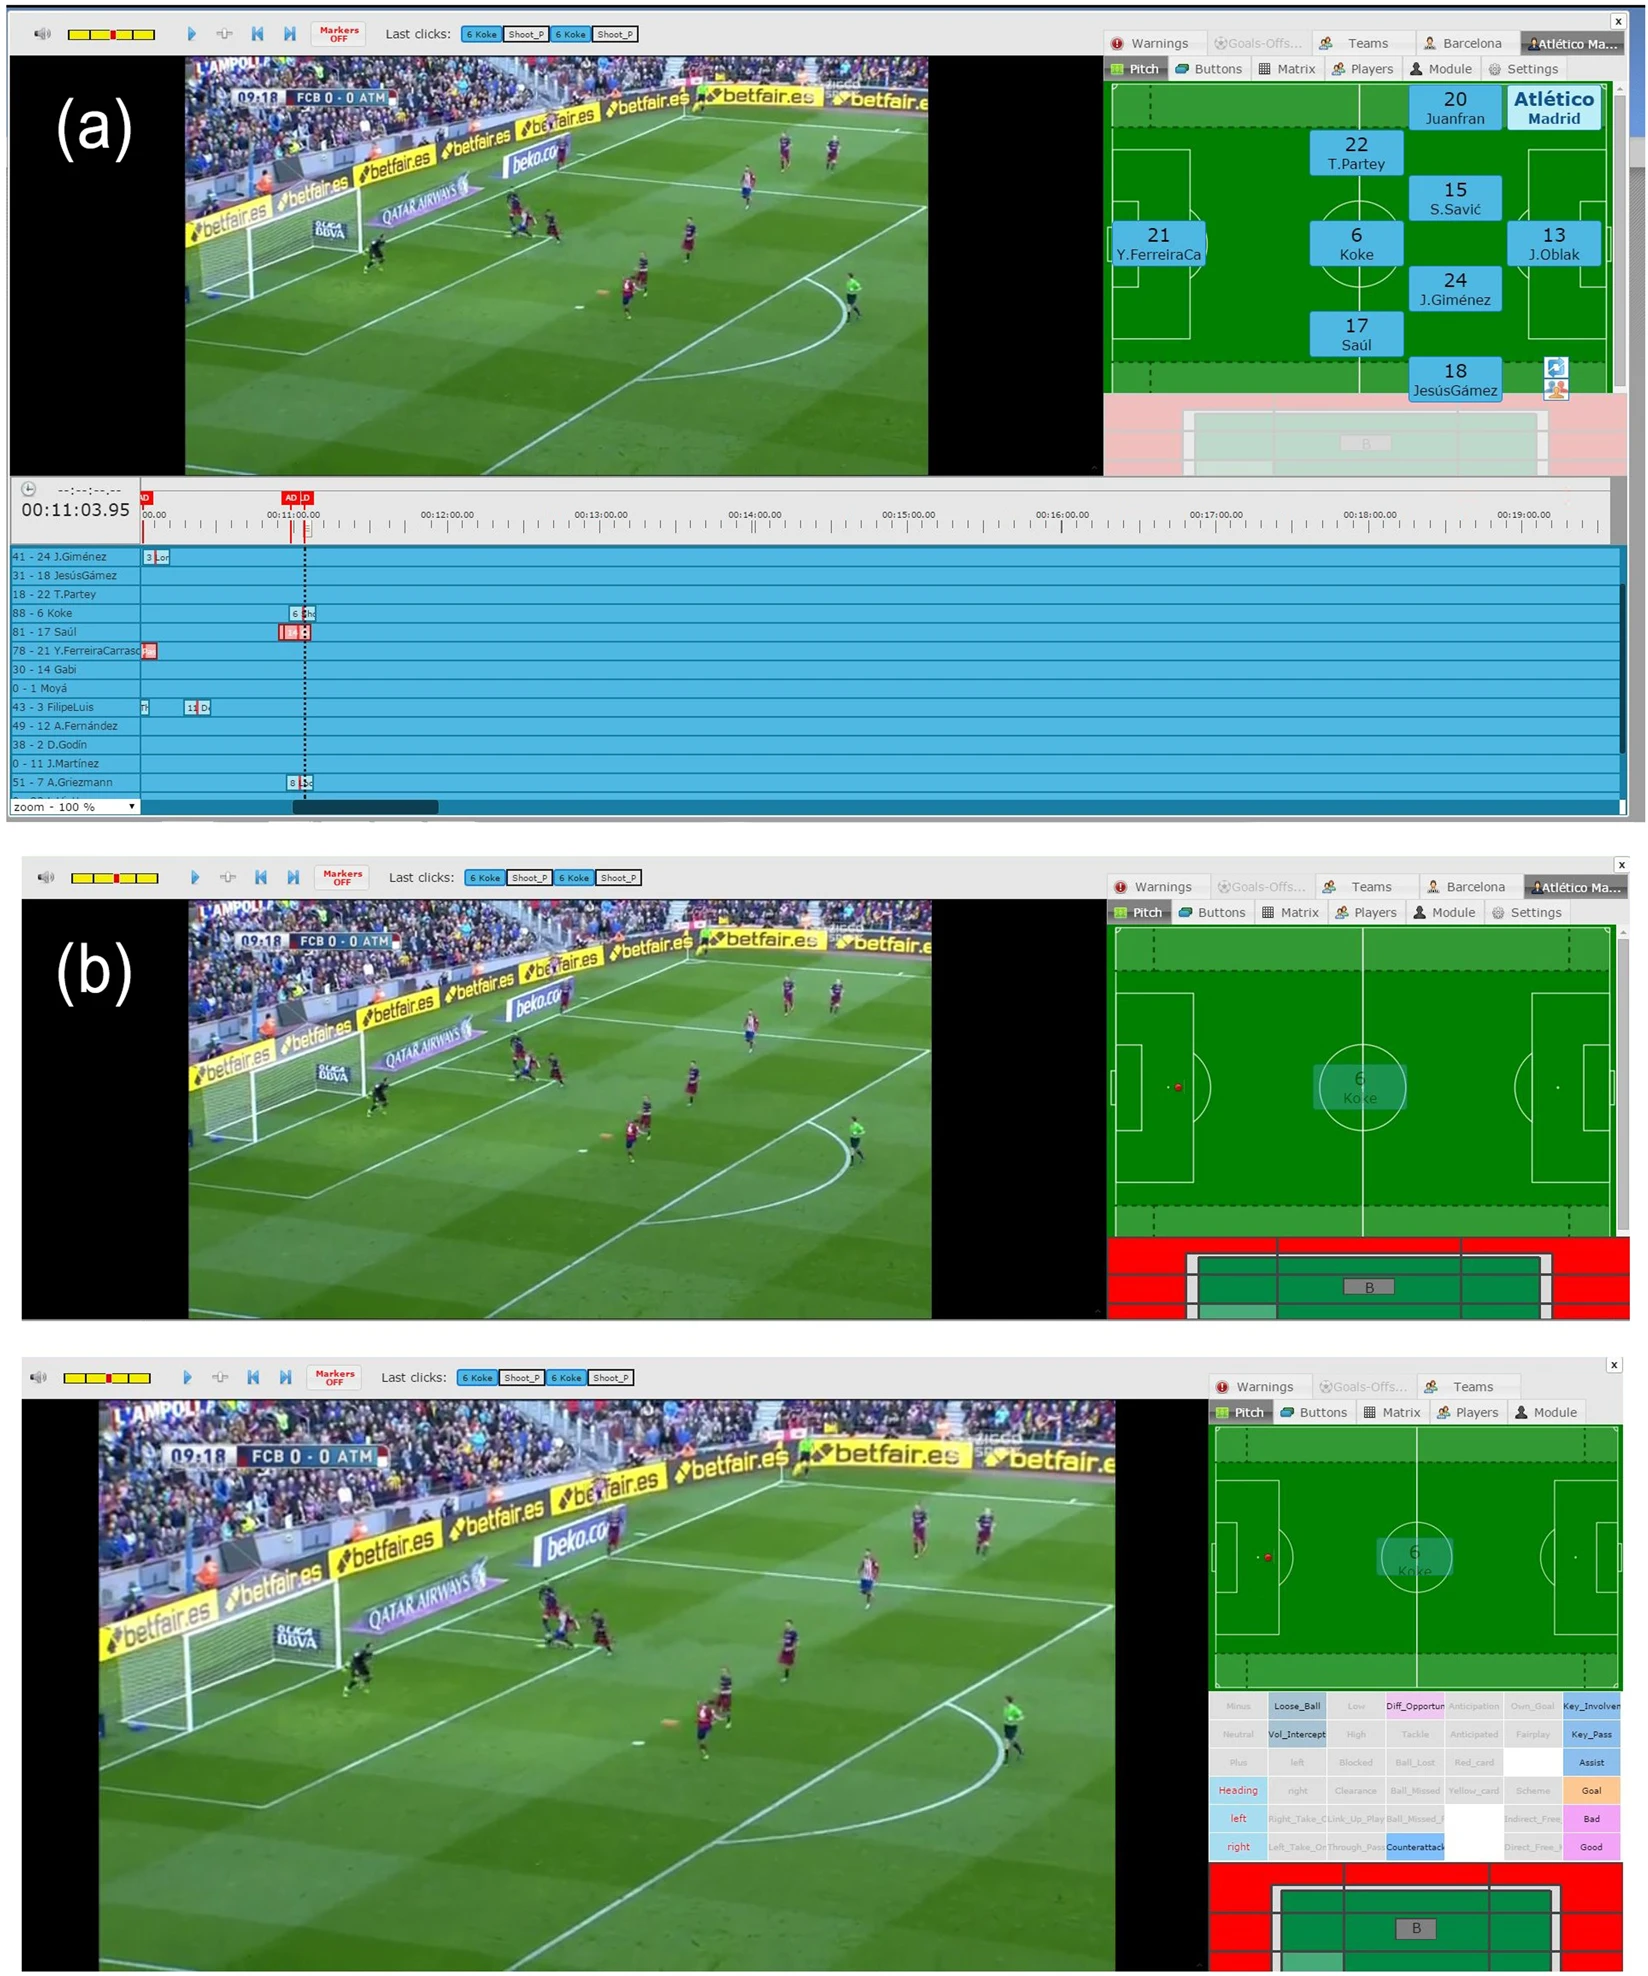
\includegraphics[width=0.7\textwidth]{img/logiciel_proprietaire.png}
    \caption{Aperçu du logiciel propriétaire de Wyscout}
    \label{fig:logiciel_proprietaire}
\end{figure}
Sur la figure \ref{fig:logiciel_proprietaire}, on peut voir un aperçu du logiciel propriétaire de Wyscout.
La partie (a) montre la timeline du match avec les événements qui ont été ajoutés.
La partie (b) montre les informations d'un événement ainsi que l'indication de la position de l'événement sur le terrain.
\newline\newline
Le dataset utilisé est un sample du dataset de Wyscout. 
Il a été mis à disposition par Luca Pappalardo et Emanuele Massuco dans leur article "A public data set of spatio-temporal match events in soccer competitions" \cite{pappalardoPublicDataSet2019}.
Ce dataset est composé des 5 championnats européens majeurs (Premier League, La Liga, Bundesliga, Serie A et Ligue 1) de la saison 2017-2018. 
Le dataset contient également les informations de la Coupe du Monde 2018 et de l'Euro 2016.
Les données sont au format JSON qui est un format très récurrent dans le monde du web. Il est également utilisé lors de communication avec des API REST.

% Description de chaque attribut dans le dataset event
\subsection{Events}
\label{subsec:events}
% Utiliser le tableau de la thèse de Luca Pappalardo
% Egalement utiliser le glossaire de Wyscout pour expliquer les tag id
Le dataset fournit par Luca Pappalardo et Emanuele Massuco contient des données sur les événements d'un match. 
Ces événements sont décrits par des attributs qui sont détaillés dans le tableau \ref{tab:events}.
\begin{table}[htp]
    \centering
    \begin{tabular}{|l|l|}
    \hline
    \textbf{Nom de l'attribut} & \textbf{Description}                                                                                                                           \\ \hline
    eventId                    & \begin{tabular}[c]{@{}l@{}}L'identifiant du type d'événement. \\ Chaque identifiant d'événement \\ est lié à un nom d'événement\end{tabular}   \\ \hline
    eventName                  & Le nom du type d'événement.                                                                                                                    \\ \hline
    subEventId                 & L'identifiant du sous-type d'événement                                                                                                         \\ \hline
    subEventName               & Le nom du sous-événement                                                                                                                       \\ \hline
    tags                       & \begin{tabular}[c]{@{}l@{}}Une liste d'événement de tag.\\ Chaque tag permet d'apporter\\ une information\end{tabular}                         \\ \hline
    eventSec                   & \begin{tabular}[c]{@{}l@{}}Le temps (en secondes) écoulé depuis\\ la période actuelle du match\end{tabular}                                    \\ \hline
    id                         & L'identifiant unique de l'événement                                                                                                            \\ \hline
    matchId                    & \begin{tabular}[c]{@{}l@{}}L'identifiant du match auquel \\ l'événement est lié.\end{tabular}                                                  \\ \hline
    matchPeriod                & \begin{tabular}[c]{@{}l@{}}La période du match à laquelle \\ l'événement a lieu.\end{tabular}                                                  \\ \hline
    playerId                   & \begin{tabular}[c]{@{}l@{}}L'identifiant du joueur qui a généré\\ l'événement. Est lié à l'attribut "wyId"\\ du dataset "Players"\end{tabular} \\ \hline
    positions                  & La localisation en X et Y de l'événement                                                                                                       \\ \hline
    teamId                     & \begin{tabular}[c]{@{}l@{}}L'identifiant de l'équipe du joueur qui a \\ généré l'événement\end{tabular}                                        \\ \hline
    \end{tabular}
    \caption{Description des attributs du dataset "Events"}
    \label{tab:events}
\end{table}

Parmi les informations fournies par le dataset, il y a "eventName".
Cet attribut permet de savoir quel type d'événement a eu lieu.
Parmi les types d'événements\footnote{Le nom des événements est en anglais mais a été traduit pour les lister}, il y a :
\begin{itemize}
    \item Passe
    \item Faute
    \item Tir 
    \item Duel
    \item Coup franc
    \item Hors-jeu
    \item Touche de balle
\end{itemize}

L'attribut "tags" est également important.
Cette attribut est une liste de tags qui permettent d'apporter des informations supplémentaires sur l'événement.
La documentation des tags peut être trouvée sur le glossaire de Wyscout. \cite{WyscoutGlossary}
Par exemple, le tag 101 indique que l'événement est un but. 
Le tag 401 indique que le tir a été fait du pied gauche, le tag 402 indique que le tir a été fait du pied droit.
Finalement, le tag 403 indique que le tir a été fait de la tête.
\newline\newline
Le dernier point important est la localisation de l'événement.
En effet, comme indiqué dans la section "Pitch coordinates" du glossaire de Wyscout, \cite{WyscoutGlossary} les coordonnées X et Y sont relatives à la taille du terrain.
Il y a un aperçu de la taille du terrain sur la figure avec ses coordonnées sur la figure \ref{fig:terrain}.
Cela donne une idée de la taille du terrain.
Le choix de la taille du terrain en 100 par 100 a été fait car les terrains n'ont pas tous la même taille malgré les règles de l'IFAB.
\newline\newline
L'IFAB est l'International Football Association Board qui est l'organisme qui définit les règles du football. 
C'est cet organisme qui définit donc la taille des terrains de football.
En effet, les terrains de football ont une taille qui peut varier entre 90 et 120 mètres de longueur et entre 45 et 90 mètres de largeur. \cite{TerrainIFAB}
\newline\newline 
Une autre information importante qui est indiqué dans la documentation de l'API de Wyscout \cite{WyscoutAPI} est que les positions des événements ont été normalisées par rapport à l'emplacement du but de l'équipe qui a généré l'événement.
Cela veut dire que dans les données fournies par le dataset, les équipes jouent toujours dans le même sens du terrain.
On peut d'ailleurs constater cela lorsqu'on regarde les positions des événements de tirs \ref{fig:events_tirs_emplacements}.
En effet sur la figure \ref{fig:events_tirs_emplacements}, on peut voir que les tirs sont toujours effectués du même côté du terrain\footnote{Certains sont effectuées dans l'autre partie du terrain mais jamais dans la surface de réparation opposée.}.
Il est également possible de visualiser la distribution des positions X des tirs sur la figure \ref{fig:histogramme_position_x_tirs}.
On voit bien que les tirs sont toujours effectués dans la même partie du terrain.
Le fait que les tirs sont relatives à la position du but de l'équipe qui a généré l'événement règle déjà un problème qui aurait pu se poser.
En effet, il aurait fallu déterminer quelle équipe joue dans quel sens du terrain et donc savoir dans quelle direction les tirs sont effectuées.
Ce travail aurait été nécessaire et extrêmement important car cela aurait pu fausser les données sur la distance et l'angle de tir.
\newline\newline
On sait donc que, dans le dataset, les équipes jouent toutes dans le même sens du terrain, Cela nous simplifie la tâche pour la suite de la thèse.

\begin{figure}[htp]
    \centering
    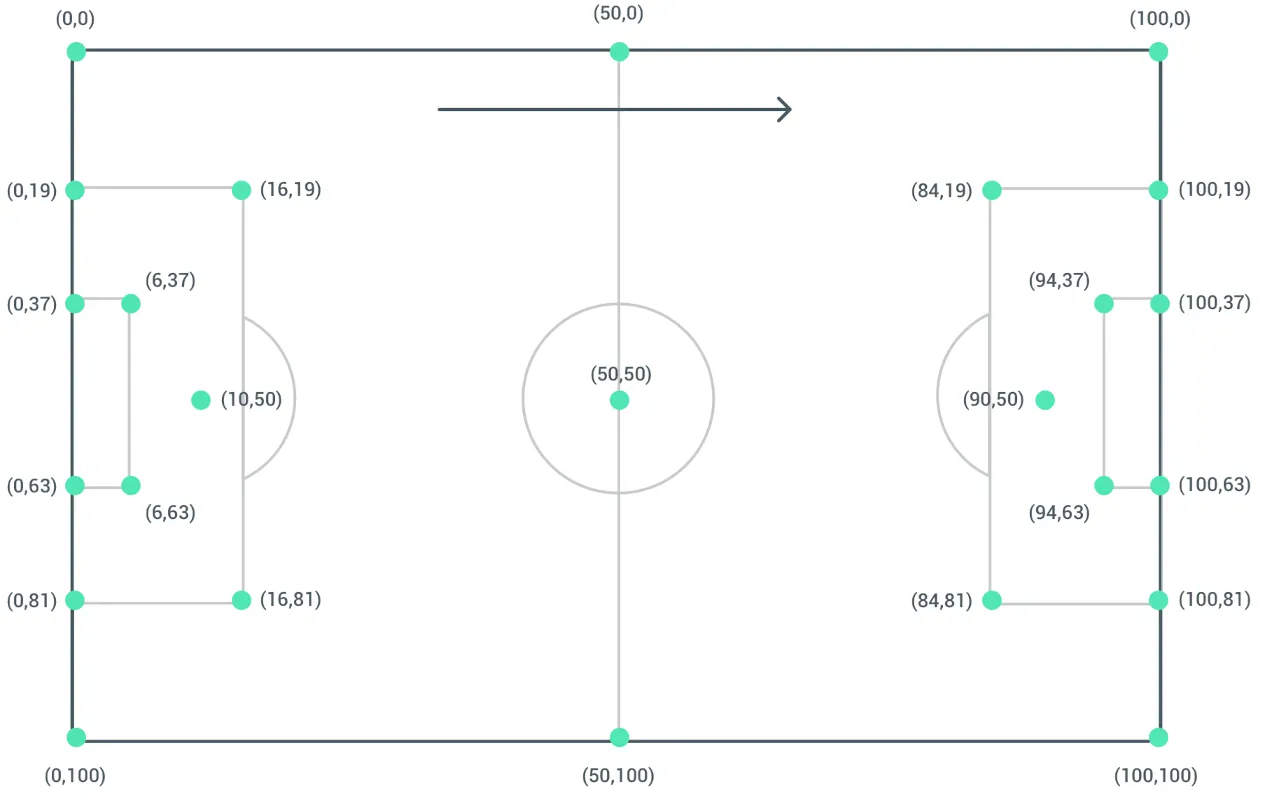
\includegraphics[width=0.8\textwidth]{img/CoordTerrain.png}
    \caption{Représentation du terrain de football avec les coordonnées X et Y}
    \label{fig:terrain}
\end{figure}

\begin{figure}[htp]
    \centering
    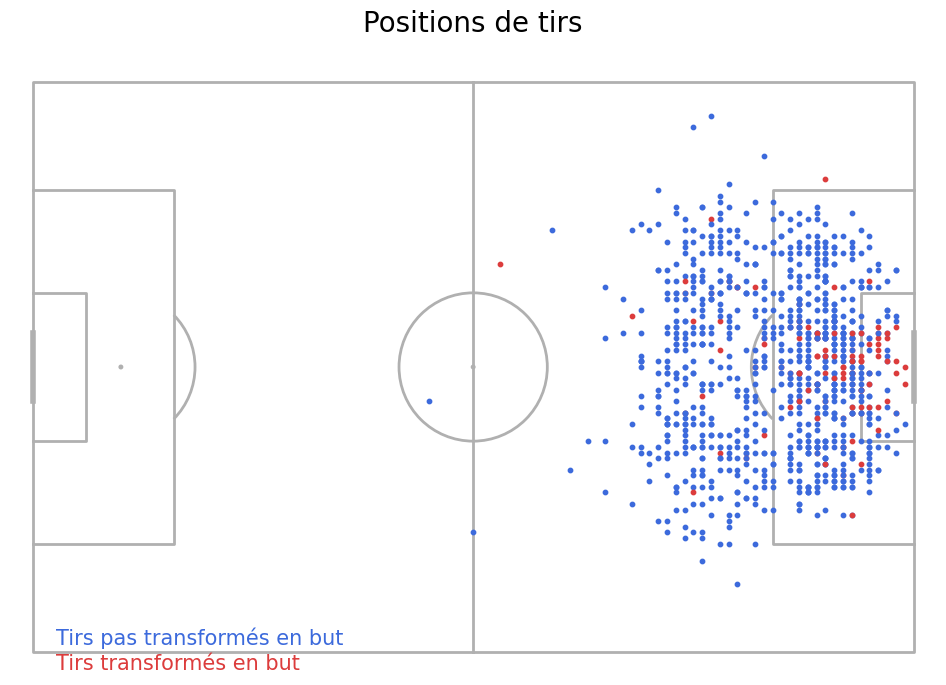
\includegraphics[width=0.8\textwidth]{img/PositionTirsDatasetEvent.png}
    \caption{Représentation des positions des 1000 premiers tirs}
    \label{fig:events_tirs_emplacements}
\end{figure}

\begin{figure}
    \centering
    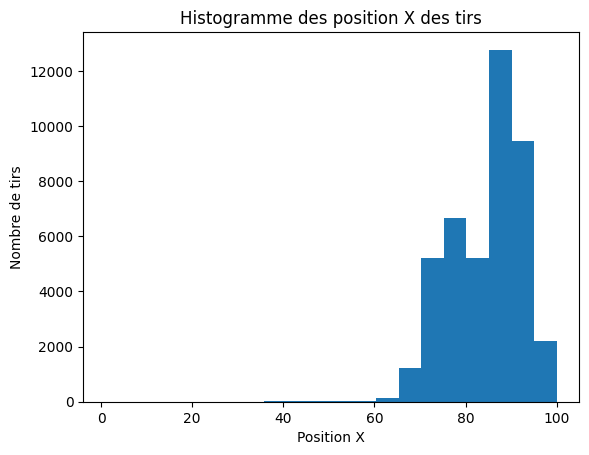
\includegraphics[width=0.8\textwidth]{img/histogramme_position_x_tirs.png}
    \caption{Histogramme des positions X des tirs}
    \label{fig:histogramme_position_x_tirs}
\end{figure}



\newpage
% Description de chaque attribut dans le dataset players
\subsection{Players}
Le dataset contient également des informations sur les joueurs.
Le tableau \ref{tab:players} décrit les attributs du dataset "Players".
\newline\newline
On peut voir que le dataset contient des informations sur les joueurs comme leur taille, leur poids, leur date de naissance, leur nationalité, leur poste, etc.
L'une des informations qui est intéressante dans la suite de la thèse et le pied fort du joueur.
En effet, le pied fort du joueur peut être un facteur qui influence le résultat de la prédiction des xG.
C'est pour cela qu'il est important de garder cet attribut dans le dataset final qui va être utilisé pour entraîner le modèle.
\begin{table}[h]
    \centering
    \begin{tabular}{|l|l|}
    \hline
    \textbf{Nom de l'attribut} & \textbf{Description}                                                                                              \\ \hline
    birthArea                  & Pays de naissance du joueur                                                                                       \\ \hline
    birthDate                  & Date de naissance du joueur                                                                                       \\ \hline
    currentNationalTeamId      & Equipe nationale du joueur                                                                                        \\ \hline
    currentTeamId              & \begin{tabular}[c]{@{}l@{}}Equipe actuelle du joueur. \\ Est lié à l'attribut "wyId" de l'équipe\end{tabular}     \\ \hline
    firstName                  & Prénom du joueur                                                                                                  \\ \hline
    lastName                   & Nom du joueur                                                                                                     \\ \hline
    foot                       & Pied fort du joueur                                                                                               \\ \hline
    height                     & Taille du joueur en centimètres                                                                                   \\ \hline
    middleName                 & \begin{tabular}[c]{@{}l@{}}Deuxième nom du joueur. S'il en \\ possède un\end{tabular}                             \\ \hline
    passportArea               & Nationalité du joueur                                                                                             \\ \hline
    role                       & Poste du joueur                                                                                                   \\ \hline
    shortName                  & Nom raccourci du joueur                                                                                           \\ \hline
    weight                     & Poids du joueur en kilogrammes                                                                                    \\ \hline
    wyId                       & \begin{tabular}[c]{@{}l@{}}Identifiant du joueur.\\ Permet de faire le lien avec le dataset "Events"\end{tabular} \\ \hline
    \end{tabular}
    \caption{Description des attributs du dataset "Players"}
    \label{tab:players}
\end{table}

\newpage
\subsection{Transformation des données}
% Parler du présupposé de la taille du terrain 105x68
% Transformation des positions des événements en angle et distance
Comme discuté dans la section \ref{subsec:events}, les coordonnées X et Y sont relatives à la taille du terrain.
Une des premiers présupposé qui est fait est que la taille du terrain est de 105 par 68.
Cette taille de terrain est la plus commune dans le football professionnel.
On peut le voir sur le site officiel de la Premier League que la taille du terrain de 105 par 68 est la plus commune. \cite{PremierLeagueClubs} 
Je démarre déjà par un présupposé que tous les terrains qui ont accueilli les matchs dans le dataset ont comme dimension 105 mètres par 68.
Ce présupposé nous permettra ainsi de pouvoir calculer la distance en mètre par rapport au but adverse ainsi que l'angle de tir.
\newpage
La première partie est de transformer les coordonnées X et Y qui sont à l'échelle 100 par 100 en coordonnées X et Y à l'échelle 105 par 68.
Pour cela, il suffit de multiplier les coordonnées X par 1.05 et les coordonnées Y par 0.68.
\begin{equation}
    \begin{split}
        x_{105} = x_{100} * 1.05 \\
        y_{68} = y_{100} * 0.68
    \end{split}
\end{equation}
On passe également les coordonnées X de l'autre côté du terrain. 
Cela permettra de calculer la distance par rapport au centre du terrain.
Il suffit de soustraire les coordonnées X à 105\footnote{Dans mon cas, j'ai soustrait les coordonnées avant de passer à l'échelle 105x68, donc j'ai soustrait les coordonnées de X à 100.}.
\newline\newline
La deuxième partie est de créer un attribut qui contient la distance par rapport au centre du terrain sur l'axe Y.
Cet attribut permettra de calculer la distance du tir ainsi que son angle.
Pour cela, il suffit de calculer la distance entre le centre du terrain et la position du tir, mais uniquement sur l'axe Y.
\begin{equation}
    \begin{split}
        y_{Centre} = \lvert y_{68} - 34 \rvert
    \end{split}
\end{equation}
34 étant la moitié de la largeur du terrain. 
Cela nous permet d'avoir la distance par rapport au centre du terrain sur l'axe Y \footnote{Pareil que pour la coordonnée X, la soustraction a été faite sur l'échelle 100x100 avant de passer à l'échelle 105x68}.
\newline\newline
La troisième partie est de calculer la distance du tir par rapport au but adverse.

Sur la figure \ref{fig:distance_tir}, [C] représente le centre du terrain, [E] représente le centre du but adverse.
[DG] représente l'attribut que l'on a calculer précédemment qui contient la distance par rapport au centre du terrain sur l'axe Y.
[DF] représente la position en X par rapport au but adverse.
Ce qui est effectué pour calculer la distance du tir par rapport au but adverse est d'utiliser le théorème de Pythagore.
On peut voir sur la figure \ref{fig:distance_tir} que l'on a un triangle rectangle [GDF].
Avec le théorème de Pythagore, on peut savoir que :
\begin{equation}
    DE^2 = GF^2 = DG^2 + DF^2
\end{equation}
Il suffit de faire une racine carré de la somme de $DG^2$ et $DF^2$ pour avoir la distance du tir par rapport au centre du but adverse.
\newline\newline
La quatrième partie est de calculer l'angle du tir par rapport au but adverse.
Il est d'abord important d'amener une autre information qui, cette fois-ci, n'est pas un présupposé.
En effet, la largeur des buts de football est de 7.32 mètres \cite{TerrainIFAB}.
Pour cette partie, le choix a été d'utiliser l'inverse de la tangente et la règle qui dit que la somme des angles d'un triangle est égale à 180 degrés.
Grâce à cela, on peut calculer l'angle du tir par rapport au but adverse.
On peut voir sur la figure \ref{fig:angle_tir} que l'on a un triangle JGF.
L'objectif est de calculer l'angle situé au sommet G.
On sait que GI représente $y_{Centre}$ et que HF représente la valeur de $x$.
FJ représente la largeur du but qui est, comme indiqué précédemment, de 7.32 mètres.
On peut donc avoir la valeur de GH et GK en additionnant ou soustrayant la moitié de la largeur du but à $y_{Centre}$.
\begin{equation}
    \begin{split}
        GH = y_{Centre} - \frac{7.32}{2} \\
        GK = y_{Centre} + \frac{7.32}{2}
    \end{split}
\end{equation}
En utilisant la tangente inverse, on peut calculer l'angle GJK ainsi que l'angle GFH.
Avec ces deux angles, on peut calculer l'angle à l'intérieur du triangle JGF pour finalement récupérer l'angle du tir par rapport au but adverse en faisant\footnote{En degrés} :
\begin{equation}
    \begin{split}
        \alpha = 180 - (Angle_{GJK} + Angle_{GFH})
    \end{split}
\end{equation}
Finalement l'équation totale ressemble à cela, une fois que l'on a toutes les valeurs :
\begin{equation}
    \begin{split}
        \alpha = 180 - (tan^{-1}(\frac{GH}{HF}) + 90) - (90 -tan^{-1}(\frac{GK}{HF}))
    \end{split}
\end{equation}

Il est d'ailleurs possible d'accéder au schémas géométrique sur Geogebra.
Cela permet de manipuler les différents points et de voir les valeurs se mettre à jour automatiquement.
Ils sont disponibles en bas de page\footnote{Angle : \url{https://www.geogebra.org/geometry/d7tqw4fe}}\footnote{Distance : \url{https://www.geogebra.org/geometry/fnx3swex}}.

\begin{figure}[htp]
    \centering
    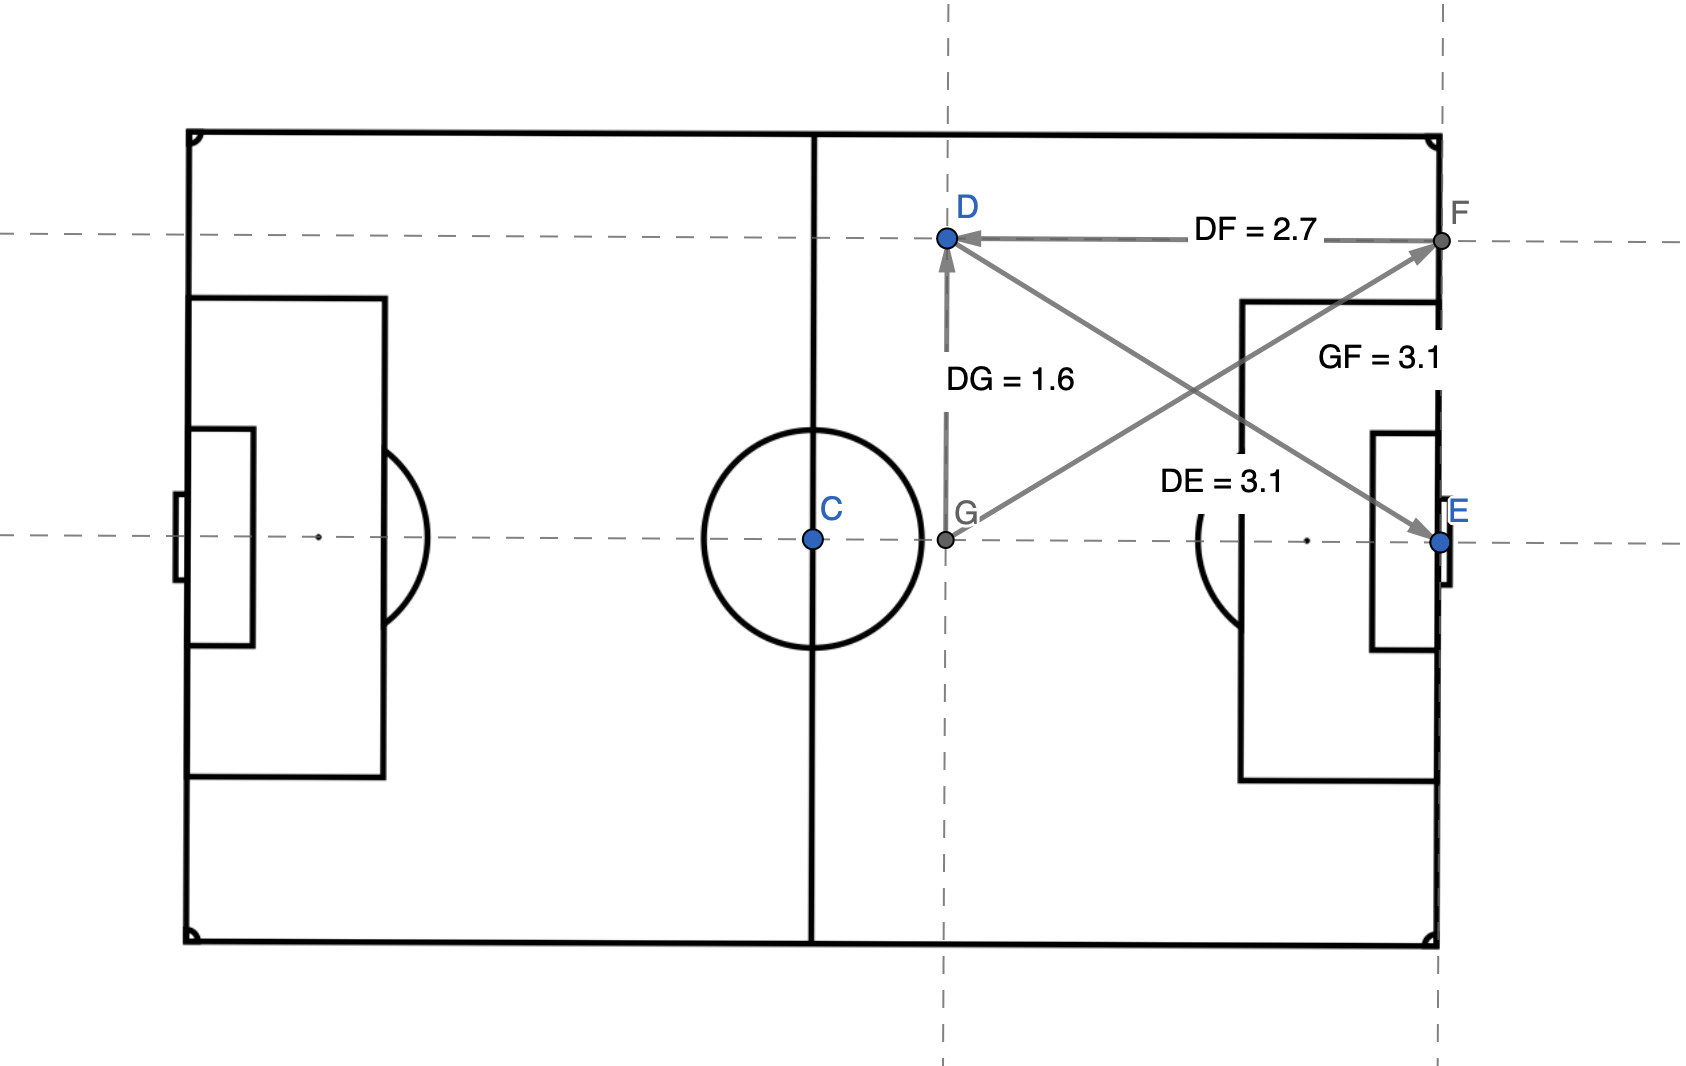
\includegraphics[width=0.9\textwidth]{img/schema_calcul_distance.png}
    \caption{Distance du tir par rapport au but adverse}
    \label{fig:distance_tir}
\end{figure}
\begin{figure}[htp]
    \centering
    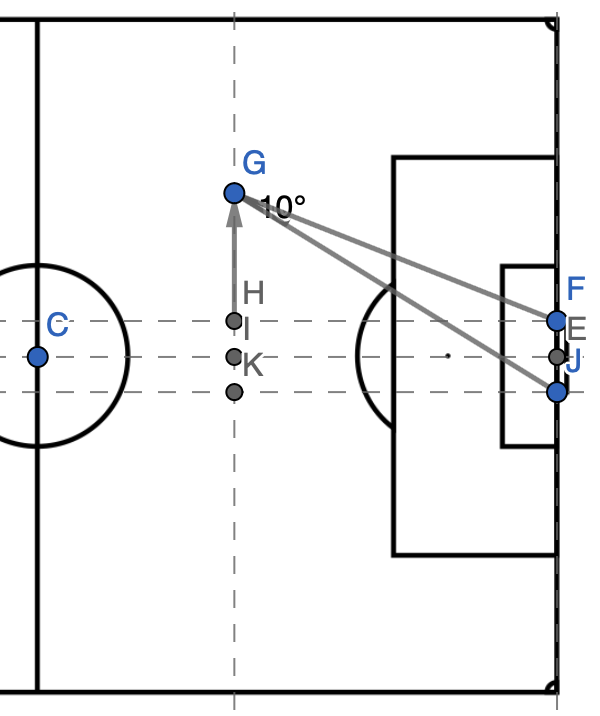
\includegraphics[width=0.5\textwidth]{img/schema_calcul_angle.png}
    \caption{Angle du tir par rapport au but adverse}
    \label{fig:angle_tir}
\end{figure}


\subsection{Fusion des datasets}
% Fusion des datasets events et players
Cette section vise à expliquer comment les datasets ont été fusionnés.
On a pu voir que le dataset events contient l'identifiant du joueur qui a effectué l'action sous le nom d'attribut "playerId" (voir table \ref{tab:events}).
Cet identifiant correspond à l'identifiant nommé "wyId" dans le dataset players (voir table \ref{tab:players}).
L'objectif est donc de fusionner les deux datasets en utilisant ce deux attributs pour permettre d'avoir les informations des joueurs dans le dataset events.
Dans notre cas, nous allons faire une jointure pour permettre de récupérer quel est le pied fort du joueur ayant généré l'événement.
Grâce à cela, il nous est possible de savoir si le joueur a tiré avec son pied fort ou non.
\newline\newline

\begin{table}[htp]
    \centering
    \begin{tabular}{|l|l|}
        \hline
        \textbf{Nom de l'attribut} & \textbf{Description}                                                                                                                   \\ \hline
        X                          & \begin{tabular}[c]{@{}l@{}}Position X sur le terrain. Permet de visualiser les \\ tirs via un pitch chart\end{tabular}                 \\ \hline
        Y                          & \begin{tabular}[c]{@{}l@{}}Position Y sur le terrain. Permet de visualiser les \\ tirs via un pitch chart\end{tabular}                 \\ \hline
        distance                   & Distance du tir par rapport au milieu du but                                                                                           \\ \hline
        angle                      & \begin{tabular}[c]{@{}l@{}}Angle des deux poteaux par rapport au tir. En \\ radians\end{tabular}                                       \\ \hline
        angle\_abs                 & L'angle du tir par rapport au centre du terrain.                                                                                                      \\ \hline
        \textbf{goal}                       & Indique si le tir est un but. \textbf{La variable cible.}                                                                                                       \\ \hline
        header                     & \begin{tabular}[c]{@{}l@{}}Indique si le tir est fait de la tête. Si c'est le cas, \\ "good\_foot\_used" est False\end{tabular}        \\ \hline
        good\_foot\_used           & \begin{tabular}[c]{@{}l@{}}Indique si le tir est fait avec le pied fort du joueur.\\ Si c'est le cas, "header" est False.\end{tabular} \\ \hline
        \end{tabular}
    \caption{Attributs du dataset events}
    \label{tab:final_dataset}
\end{table}

\subsection{Visualisation des données}
% Visualisation des données
Cette section vise à visualiser les données du dataset final.
Tout d'abord, nous allons effectuer une description simple du dataset.
Le dataset contient 43075 tirs sur une saison de football (2017/2018) dans 7 compétitions différentes :
\begin{itemize}
    \item Ligue 1
    \item Premier League
    \item Serie A
    \item Bundesliga
    \item La Liga
    \item Coupe du monde 2018
    \item Euro 2016
\end{itemize}
La description du dataset est disponible sur le tableau \ref{tab:describe_dataset}.
On peut voir que la distance maximale d'un tir a été de 103.95 mètres et la distance minimale de 0.68 mètre.
On constate donc que certains tirs n'ont pas été normalisés par rapport au sens du jeu de l'équipe comme indiqué dans la section \ref{subsec:events}. 
C'est pour cela que notre but va être de retirer certains tirs considérés comme des "outliers".
\begin{table}[htp]
    \centering
    \begin{tabular}{r|r|r|r|r|r|}
        \cline{2-6}
        \textbf{}                   & \textbf{X}   & \textbf{Y}   & \textbf{distance} & \textbf{angle} & \textbf{angle\_abs} \\ \hline
        \multicolumn{1}{|r|}{count} & 43075 & 43075 & 43075      & 43075   & 43075        \\ \hline
        \multicolumn{1}{|r|}{mean}  & 15.992225    & 33.473176    & 18.593067         & 0.414140       & 2.657552            \\ \hline
        \multicolumn{1}{|r|}{std}   & 8.534333     & 9.366171     & 8.419298          & 0.253173       & 0.313051            \\ \hline
        \multicolumn{1}{|r|}{min}   & 0.000000     & 0.000000     & 0.680000          & 0.000000       & 1.570796            \\ \hline
        \multicolumn{1}{|r|}{25\%}  & 9.450000     & 26.520000    & 12.249445         & 0.250188       & 2.441817            \\ \hline
        \multicolumn{1}{|r|}{50\%}  & 13.650000    & 33.320000    & 17.153297         & 0.327782       & 2.689439            \\ \hline
        \multicolumn{1}{|r|}{75\%}  & 23.100000    & 40.800000    & 24.936000         & 0.505984       & 2.914297            \\ \hline
        \multicolumn{1}{|r|}{max}   & 103.950000   & 68.000000    & 103.952224        & 3.141593       & 3.141593            \\ \hline
        \end{tabular}
    \caption{Description du dataset final}
    \label{tab:describe_dataset}
\end{table}
Pour cela, nous allons utiliser un pitch chart.
Un pitch chart est un graphique qui affiche un terrain de football.
Grâce à cela on peut visualiser plus simplement d'où ont été effectuées les tirs.
Le but de notre pitch chart est de visualiser les tirs qui ont été effectués à leurs positions respectives.
Dans mon cas, j'ai décidé d'utiliser une heatmap pour visualiser la fréquence des tirs à chacune des positions sur le terrain.
Le pitch chart peut être vu sur la figure \ref{fig:pitch_chart}.
On peut voir qu'une grande majorité des tirs ont été effectués dans la surface de réparation.
On peut également remarquer qu'il y a très peu de tirs à l'entrée de la surface de réparation.
Il y a plusieurs hypothèses qui peuvent être faites pour expliquer cela.
La première est que les joueurs préfèrent tirer dans la surface de réparation car ils ont plus de chances de marquer. 
Cependant, on remarque qu'il y a également des tirs plus lointain.
La deuxième hypothèse est que ce phénomène est dû à comment les données sont récoltées.
Il est effectivement possible que les opérateurs ou que le logiciel propriétaire de Wyscout détermine qu'un tir ait été fait dans la surface de réparation ou en dehors de celle-ci, plutôt que sur la ligne de la surface de réparation.
Cela nous montre déjà une des limitations des données que nous utilisons.
\begin{figure}[htp]
    \centering
    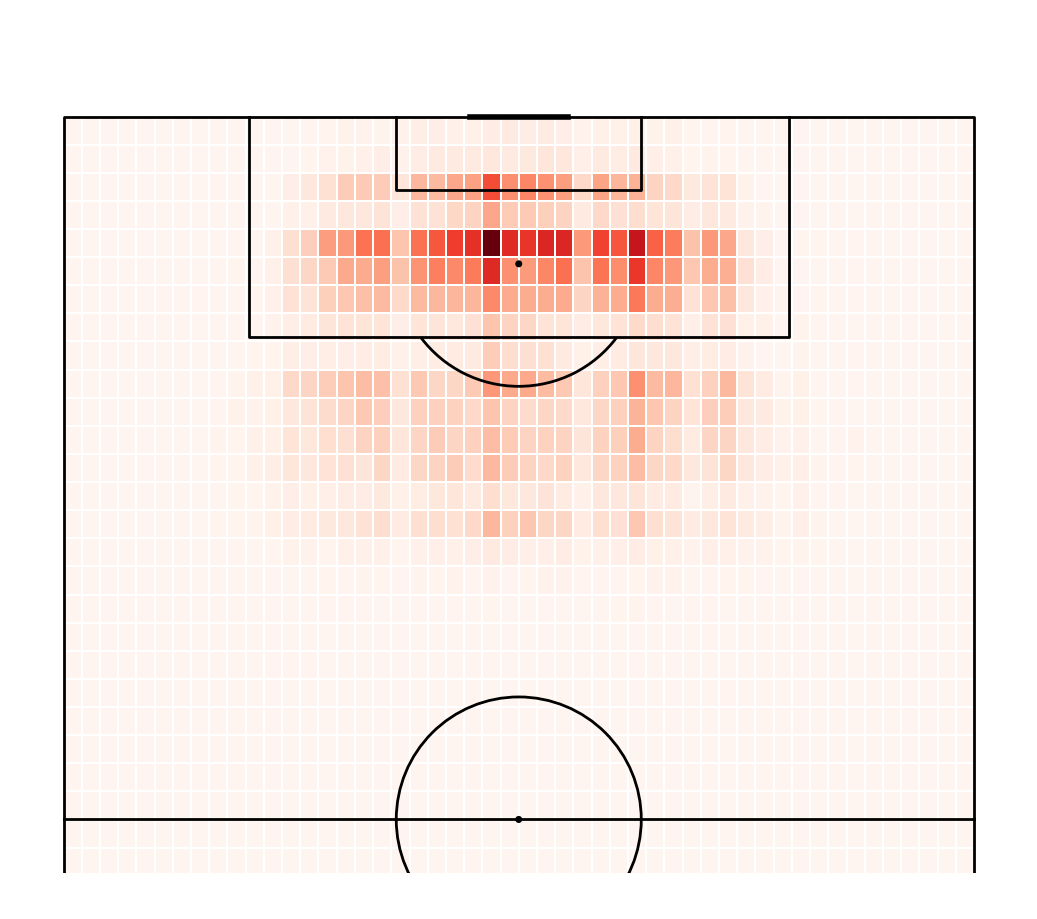
\includegraphics[width=0.8\textwidth]{img/pitchChartFrequency.png}
    \caption{Pitch chart des tirs effectués}
    \label{fig:pitch_chart}
\end{figure}

Maintenant, nous allons nous focaliser sur la détection d'éventuelles "outliers".
En effet, nous avons pu voir que la distance maximale d'un tir a été de 103.95 mètres. 
Il faut donc vérifier si ce tir est un "outlier" ou non. 
Nous allons également nous focaliser sur d'autres tirs considérés comme "outliers".
Tout d'abord, visualisons les graphiques de la distance, l'angle de tir et l'angle de tir absolu (voir fig. \ref{fig:analyse_quantitative}).
Lorsque l'on observe les histogrammes, on remarque que pour la distance et l'angle de tir, il y a une majorité de tirs qui ont été effectués à une distance inférieure à 50 mètres et un angle de tir inférieur à 1.5 radian.
On peut également voir qu'il n'y a pas de séparation distincte entre les distributions des tirs selon leur valeur cible via les graphiques de la deuxième colonne.
Cela aurait été très pertinent puisque l'on aurait pu voir quel attribut aurait été le plus influent directement en observant les données.
Cependant, on peut remarquer que des outliers ont été trouvés pour la distribution des différentes variables via les boxplots. 
Les outliers sont déterminées en se basant sur la règle suivante \cite{galarnykUnderstandingBoxplotsHow2022} :
\begin{equation}
    \begin{split}
        x < Q_1 - 1.5 * IQR \\
        x > Q_3 + 1.5 * IQR    
    \end{split}
\end{equation}
Comme indiqué sur la documentation de Matplotlib concernant les boxplots \cite{MatplotlibPyplotBoxplot}, la valeur de 1.5 est une valeur basée sur la définition initiale des boxplots de John Tukey.
Ils permettent de définir les "maximum non-outlier" et "minimum non-outlier".
\newline
Via cette formule, on peut récupérer tous les outliers pour chaque variable, on obtient donc un tableau comme celui-ci (voir tab. \ref{tab:outliers}):
L'objectif est maintenant de visualiser la probabilité de chacun des sets d'outliers. 
Si l'on observe des anomalies ou des données aberrantes, il faudra les supprimer.
\begin{table}[htp]
    \centering
    \begin{tabular}{l|l|l|l|}
        \cline{2-4}
        \multicolumn{1}{r|}{}                                                             & \textbf{Distance} & \textbf{Angle} & \textbf{Angle absolu} \\ \hline
        \multicolumn{1}{|l|}{\begin{tabular}[c]{@{}l@{}}Nombre\\ d'outliers\end{tabular}} & 197               & 2163           & 70                    \\ \hline
    \end{tabular}
    \caption{Nombre d'outliers pour chaque variable quantitatives}
    \label{tab:outliers}
\end{table}

Grâce à la figure \ref{fig:analyse_outlier2}, plusieurs observations peuvent être faites. 
Tout d'abord, il est remarquable que les outliers pour les angles ne sont pas aberrants. 
En effet, théoriquement, plus l'angle est grand, plus le but est facile à réaliser. 
Cependant, en ce qui concerne les distances, il existe un nombre très limité d'outliers. 
En examinant les valeurs situées entre 90 et 105, on constate que trois buts ont été marqués à cette distance. 
En revanche, le nombre de tirs manqués dans la même plage est plus élevé.
Théoriquement, marquer un but à 90 mètres du but est considéré comme irréalisable. 
Par conséquent, ces données peuvent être considérées comme aberrantes et il serait envisageable de les supprimer. 
Une hypothèse plausible est que ces données n'ont pas été correctement traitées par Wyscout lors de la normalisation des positions des tirs.
\newline\newline
Il est également intéressant d'examiner la relation entre la distance et l'angle. 
La figure \ref{fig:analyse_qualitative} met en évidence le fait que plus la distance est petite, plus l'angle est grand. 
Cette tendance est observée dans le premier graphique de la figure \ref{fig:analyse_qualitative}, bien que ce ne soit pas toujours le cas. 
En jouant avec le graphique Geogebra fourni précédemment, il est possible de constater que les tirs effectués depuis le coin de l'équipe attaquante auront un angle plus élevé que les tirs effectués depuis le coin de l'équipe adverse.
Un tir depuis le coin de l'équipe adverse aura systématiquement un angle de 0 radian puisqu'il est effectué le long de la ligne de but.
\newline\newline
Ensuite, nous allons analyser les attributs qualitatifs en utilisant des diagrammes en barres (bar charts). 
Ces graphiques permettent de visualiser la distribution des données pour chaque attribut qualitatif. 
Ils sont présentés dans la figure \ref{fig:analyse_qualitative}. 
À travers ces bar charts, il est possible d'observer que 10\% des tirs sont des buts. 
On remarque également qu'il y a une majorité de tirs effectués avec le pied fort du tireur. 
Cependant, les tirs qui ne sont pas effectués avec le pied fort incluent également les tirs de la tête.
Environ 15\% des tirs sont réalisés de cette manière, ce qui indique que la majorité des tirs sont effectués avec le pied (faible ou fort).
\newline\newline
Enfin, nous allons analyser la corrélation entre les variables.
L'objectif de cette analyse est d'évaluer si les variables sont corrélées les unes avec les autres.
Pour rappel, deux variables sont corrélées si elles ont tendance à varier ensemble. 
Une corrélation négative indique que lorsque la valeur d'une variable augmente, la valeur de l'autre variable diminue. 
Une corrélation positive indique que lorsque la valeur d'une variable augmente, la valeur de l'autre variable augmente également. 
Une corrélation élevée entre une variable et la variable cible peut améliorer la prédiction et faciliter l'interprétation du modèle. 
Une corrélation élevée suggère une relation claire entre les deux variables, ce qui peut faciliter la compréhension de l'influence de la variable sur la variable cible.
\newline\newline
Dans notre cas, en observant la figure \ref{fig:correlation_matrix}, les variables présentant la corrélation la plus élevée par rapport à l'attribut "goal" sont les attributs "distance" et "angle". 
Nous remarquons également une forte corrélation entre les attributs "distance" et "X". 
Cette corrélation s'explique par le fait que l'attribut "distance" est une variable dérivée de l'attribut "X" et de l'attribut "C" qui est elle-même dérivée de l'attribut "Y".
\begin{figure}[htp]
    \centering
    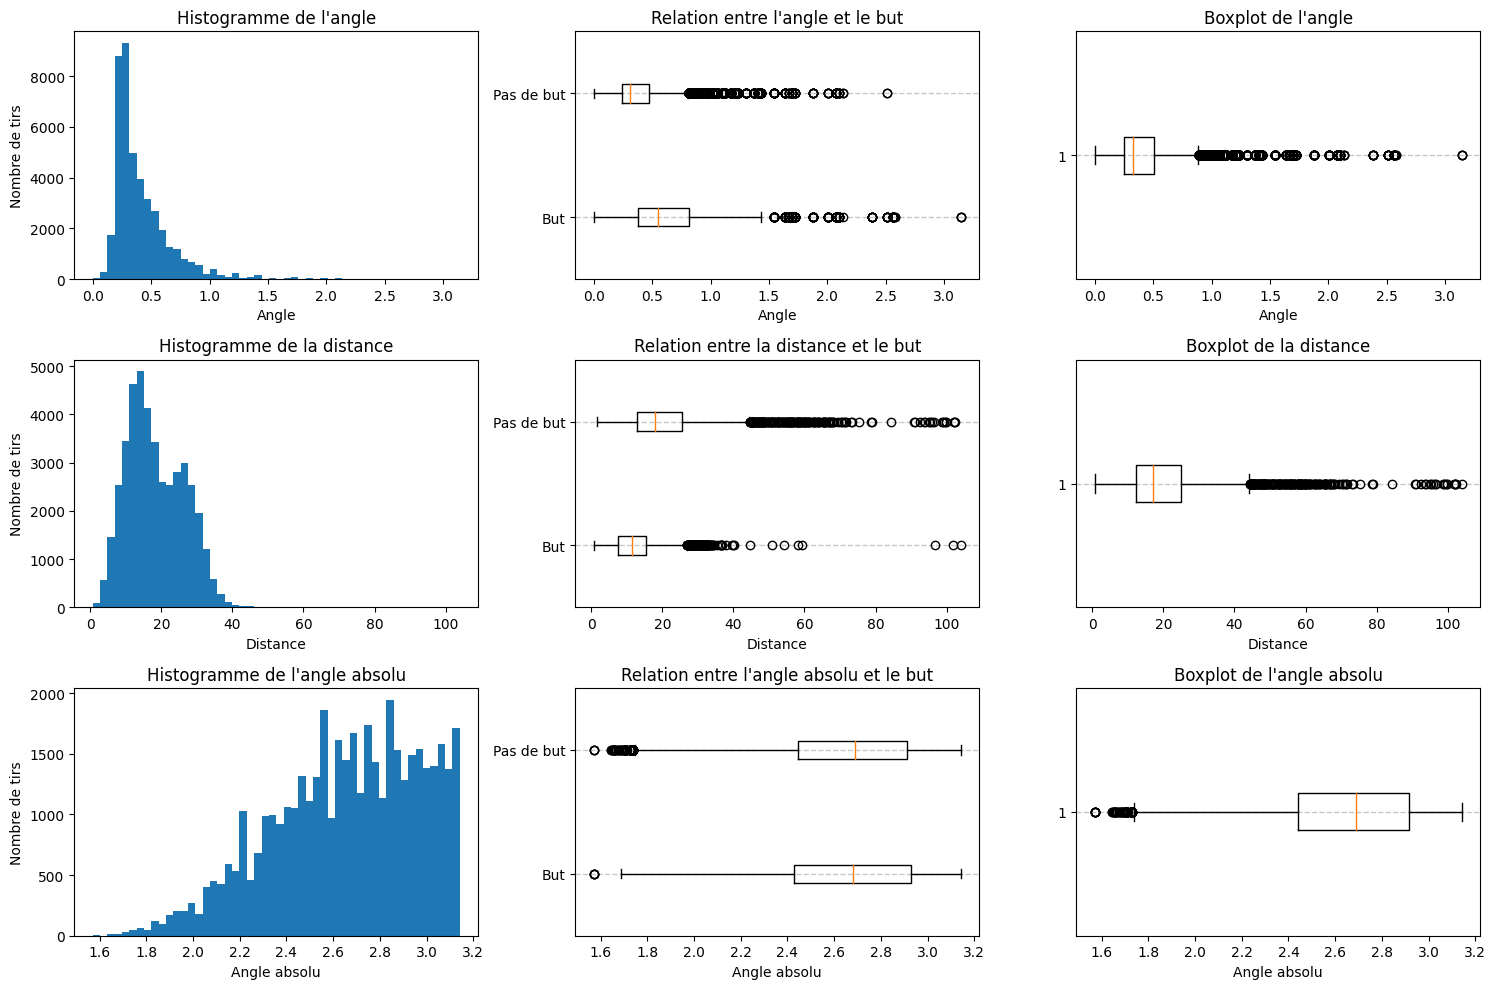
\includegraphics[width=\textwidth]{img/analyseOutlier.png}
    \caption{Analyse des attributs quantitatifs}
    \label{fig:analyse_quantitative}
\end{figure}

\begin{figure}[htp]
    \centering
    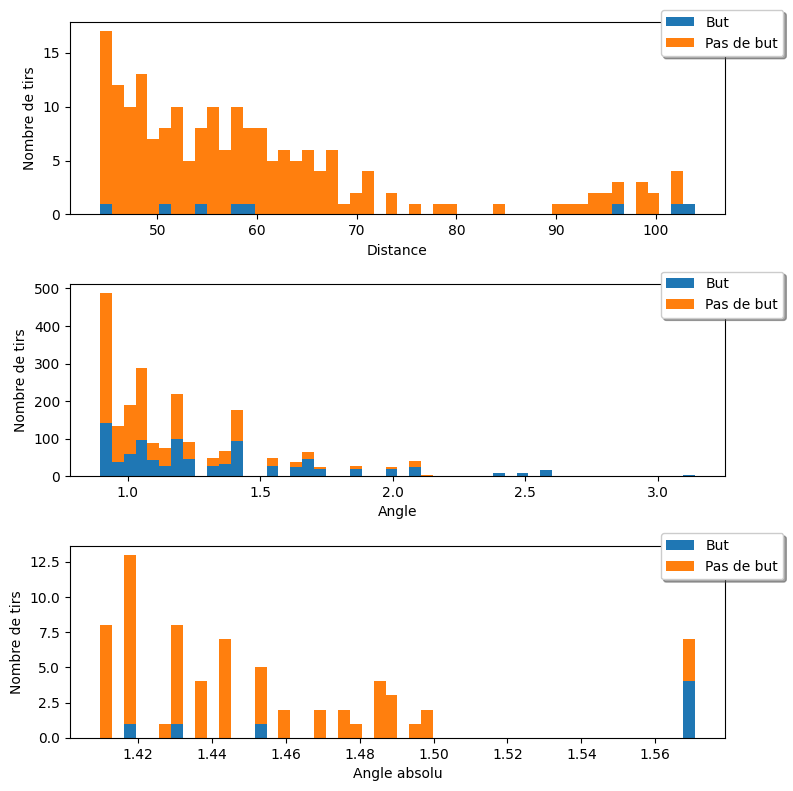
\includegraphics[width=\textwidth]{img/analyseOutlier2.png}
    \caption{Analyse des outliers}
    \label{fig:analyse_outlier2}
\end{figure}
\begin{figure}[htp]
    \centering
    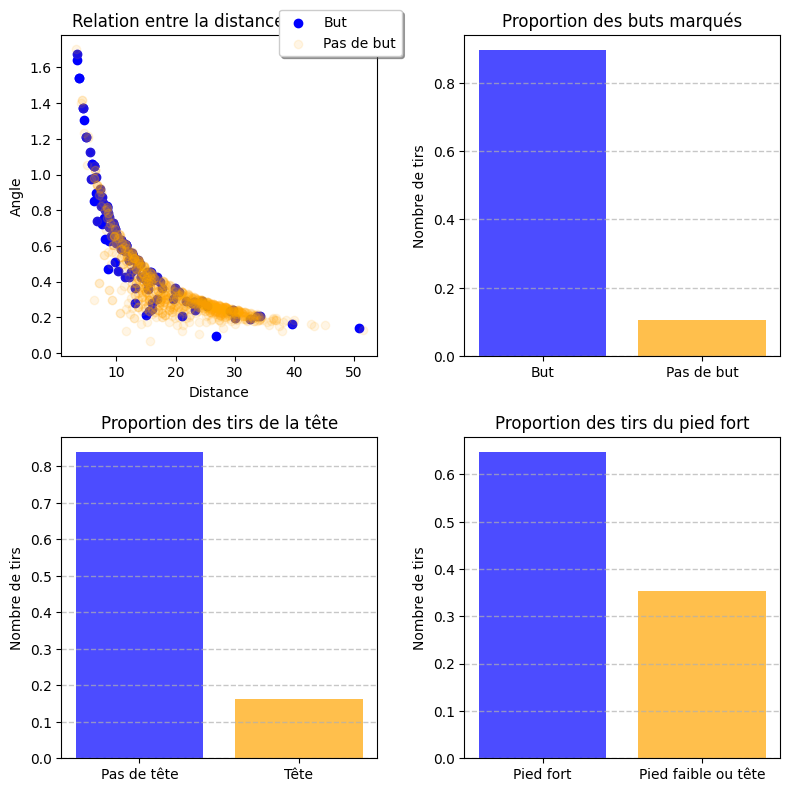
\includegraphics[width=\textwidth]{img/visualisation_discret.png}
    \caption{Relation distance-angle et analyse des attributs qualitatifs}
    \label{fig:analyse_qualitative}
\end{figure}

\begin{figure}
    \centering
    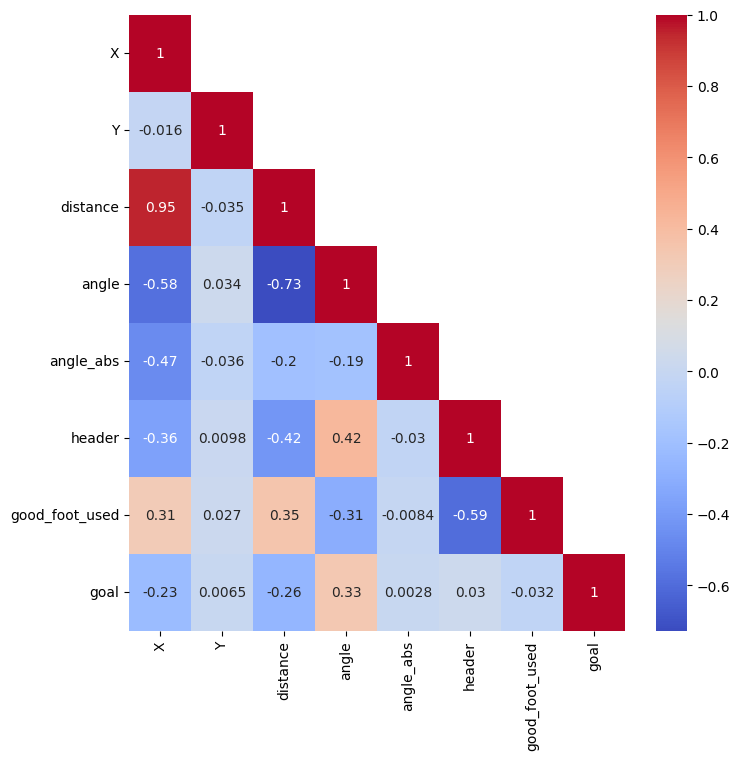
\includegraphics[width=\textwidth]{img/correlation_matrix.png}
    \caption{Matrice de corrélation des attributs}
    \label{fig:correlation_matrix}
\end{figure}
\newpage
Grâce à cette visualisation approfondie, nous avons pu acquérir une compréhension approfondie des données et des relations entre les différentes variables. 
Nous avons également identifié certaines données incohérentes et des aberrations dans le jeu de données. 
Ces observations soulignent l'importance de l'examen attentif et critique des données afin d'éliminer les valeurs aberrantes et d'obtenir des résultats plus fiables.
\newline\newline
En analysant les corrélations entre les variables, nous avons constaté que certaines d'entre elles présentaient une forte corrélation avec la variable cible. 
Cela suggère que ces variables sont des indicateurs significatifs pour prédire la réussite d'un tir au but. 
Par exemple, les variables "distance" et "angle" ont montré une corrélation élevée avec la variable "goal". 
Cela signifie que plus la distance et l'angle sont favorables, plus la probabilité de marquer un but est élevée. 
\newline\newline
Il est également important de souligner la forte corrélation entre les variables "distance" et "X". 
Cette corrélation s'explique par le fait que l'attribut "distance" est calculé en utilisant les coordonnées horizontales "X" et "C". 
Ainsi, lorsque la valeur de l'attribut "X" change, cela influence directement la valeur de l'attribut "distance". 
\newline\newline
En résumé, cette analyse approfondie des données nous a permis de mieux comprendre les relations entre les variables et d'identifier les facteurs les plus pertinents pour prédire la réussite d'un tir au but. 
En éliminant les données aberrantes et en tenant compte des corrélations significatives, nous pouvons améliorer la précision des prédictions.
Cependant, il convient de noter que des analyses supplémentaires et des modélisations plus avancées peuvent être nécessaires pour tirer des conclusions plus précises et éclairantes.

\newpage
% Affichage de la visualisation suite au retour de Nils

\section{Méthodologie}
% Liste des méthodes qui vont être utilisées
Dans cette section, nous allons discuter de la méthodologie utilisée pour résoudre le problème de prédiction de la réussite d'un tir au but.
Tout d'abord, nous allons faire une séparation sur le dataset pour avoir un jeu de données d'entraînement et un jeu de données de test.
Le jeu de tests sera utilisé pour évaluer la performance des modèles finaux. 
Tandis que le jeu d'entraînements, nous permettra d'entraîner notre modèle et de choisir le meilleur set d'hyper paramètres pour chaque modèle.
Le partitionnement choisi pour les jeux de données est le suivant : 90\% des données pour le jeu d'entraînement et 10\% des données pour le jeu de test.

\subsection{Choix des modèles}
Plusieurs modèles vont être utlisés pour résoudre ce problème.
Nous allons utiliser des modèles de classification binaire, car nous cherchons à prédire si un tir au but est réussi ou non.
Je rappelle également que le but de la thèse est de répondre à la question suivante : "Quels sont les paramètres qui influencent le plus l'expected goal ?".
Certains de ces modèles ne seront pas les plus performants et les plus cohérents pour avoir la meilleure prédiction possible mais ils permettront de comprendre les paramètres qui influencent le plus l'expected goal.
Nous allons tester les modèles suivants :
\begin{itemize}
    \item Régression logistique
    \item Arbre de décision
    \item Random Forest
    \item SVM
    \item Réseau de neurones 
\end{itemize}


\subsection{Cross Validation}
Pour chaque modèle, nous allons utiliser la cross validation pour choisir le meilleur set d'hyper paramètres.
La cross validation est une méthode qui permet de tester la performance d'un modèle sur un jeu de données.
Elle consiste à séparer le jeu de données en plusieurs sous-ensembles.
Comme on peut le voir sur la figure \ref{fig:cross_validation}, le jeu de données est séparé en 5 sous-ensembles.
Chaque itération consiste à entraîner le modèle sur 4 sous-ensembles et à tester le modèle sur le dernier sous-ensemble.
Cette opération est répétée 5 fois pour que chaque sous-ensemble soit utilisé comme jeu de test.
La performance du modèle est calculée en faisant la moyenne des performances obtenues sur chaque sous-ensemble.
C'est ainsi que nous pouvons choisir le meilleur set d'hyper paramètres pour chaque modèle.
\newline\newline
Après avoir choisi nos modèles et leurs hyper paramètres, nous allons les entraîner sur le jeu de données d'entraînement entier et les tester sur le jeu de données de test.
Cela nous permettra ensuite de comparer les résultats entre les différents modèles.
Le but est d'avoir la meilleure version d'un modèle et de la comparer avec la meilleure version des autres modèles. 
C'est ainsi que l'on pourra déterminer quel modèle est le plus performant pour résoudre notre problème.
\begin{figure}[htp]
    \centering
    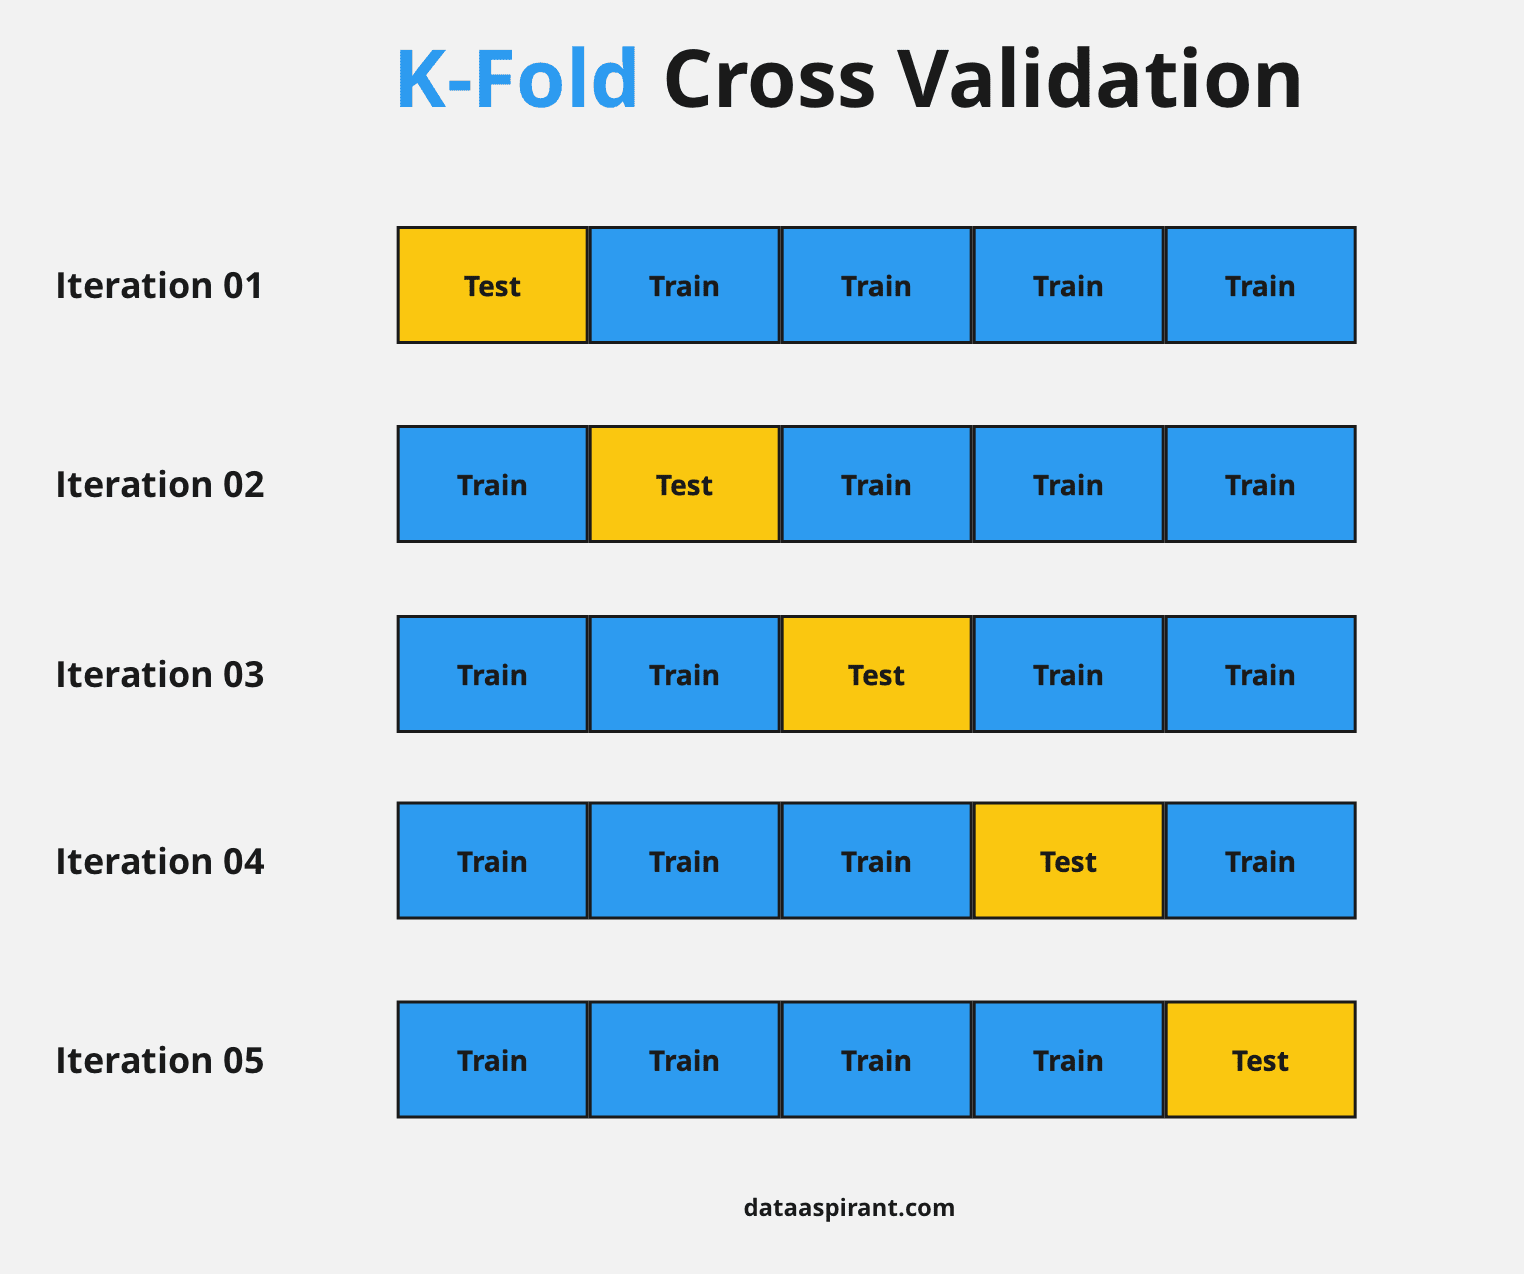
\includegraphics[width=0.6\textwidth]{img/cross_validation_schema.png}
    \caption{Cross Validation - Source : Dataspirant}
    \label{fig:cross_validation}
\end{figure}

\subsection{Sélection des meilleurs attributs}
Pour la sélection des meilleurs attributs, nous allons utiliser la méthode de forward elimination.
Cette méthode consiste à tester tous les attributs un par un en les ajoutant au fur et à mesure au modèle et observer la performance du modèle.
La p-value est utilisée pour déterminer si un attribut est significatif ou non et s'il apporte une amélioration à la performance du modèle.
Plus la p-value est faible, plus l'attribut est significatif.
\newline\newline
Par exemple, dans le tableau \ref{tab:logistic_regression_result_1}, on peut voir que l'attribut "X" a une p-value de 0.000.
Cela indique que cet attribut est significatif et qu'il apporte une amélioration à la performance du modèle en plus de la constante.
\newline\newline
Sur le tableau \ref{tab:logistic_regression_result_2}, on peut voir que l'attribut "Y" a une p-value de 0.960.
Cela indique que cet attribut n'est pas du tout significatif et qu'il n'apporte aucune amélioration à la performance du modèle.
On le remarque d'ailleurs lorsque l'on observe la valeur du coefficient qui est très proche de 0.
Il faut donc supprimer cet attribut du modèle.
\newline\newline
Pour la troisième itération sur le tableau \ref{tab:logistic_regression_result_3}, on ajoute l'attribut "distance" au modèle.
Cependant, on a supprimé l'attribut "Y" qui n'était pas significatif.
On remarque donc que les p-values des attributs "X" et "distance" sont très faibles.
Cela indique que ces deux attributs sont significatifs et qu'ils apportent une amélioration à la performance du modèle.
La valeur du coefficient de l'attribut "distance" est négative. 
Cela veut dire que plus la distance est grande, plus la probabilité d'avoir un but est faible.
\newline\newline
Pour la quatrième itération sur le tableau \ref{tab:logistic_regression_result_4}, on ajoute l'attribut "angle" au modèle.
Cependant, dans ce cas-ci, on observe que la p-value de l'attribut "X" est très élevée. 
Cela est dû à la corrélation entre les attributs "X" et "angle" qui est répétitive dû à la corrélation avec l'attribut "distance".
C'est pour cela que l'attribut "X" n'est plus significatif et qu'il n'apporte plus d'amélioration à la performance du modèle.
C'est justement dû au fait que l'attribut "distance" et l'attribut "angle" sont des attributs dérivés de l'attribut "X" et de l'attribut "Y".
\newline\newline
Lors de la cinquième itération, on ajoute l'attribut "angle\_abs" au modèle.
Ici, on observe que la p-value de l'attribut "angle\_abs" est très élevée.
Cela est dû à la corrélation entre les attributs "angle" et "angle\_abs" qui est répétitive.
C'est pour cela que l'attribut "angle\_abs" n'est pas significatif et qu'il doit être retiré.
\newline\newline
Pour finir, on peut voir sur le tableau \ref{tab:logistic_regression_result_6} que l'ajout de l'attribut "header" et "good\_foot\_used" apporte une amélioration significative au modèle.
Cela se voit grâce aux p-values très faibles de ces deux attributs lorsqu'on les ajoute aux autres attributs du modèle.


\begin{table}[htp]
    \centering
    \begin{tabular}{lllllll}
        \multicolumn{7}{c}{\textbf{Logistic Regression Result}}                        \\ \hline
              & coef    & std err & z       & P\textgreater{}|z| & {[}0.025 & 0.975{]} \\ \hline
        const & -0.4809 & 0.037   & -13.120 & 0.000              & -0.553   & -0.409   \\
        X     & -0.1280 & 0.003   & -42.743 & 0.000              & -0.134   & -0.122   \\ \hline
        \end{tabular}
    \caption{Résultat de la régression logistique - 1ère itération}
    \label{tab:logistic_regression_result_1}
\end{table}
\begin{table}[htp]
    \centering
    \begin{tabular}{lllllll}
    \multicolumn{7}{c}{\textbf{Logistic Regression Result}}                          \\ \hline
          & coef      & std err & z       & P\textgreater{}|z| & {[}0.025 & 0.975{]} \\ \hline
    const & -0.4843   & 0.076   & -6.334  & 0.000              & -0.634   & -0.334   \\
    X     & -0.1280   & 0.003   & -42.729 & 0.000              & -0.134   & -0.122   \\
    Y     & 9.939e-05 & 0.002   & 0.050   & 0.960              & -0.004   & 0.004   \\ \hline
    \end{tabular}
    \caption{Résultat de la régression logistique - 2ème itération}
    \label{tab:logistic_regression_result_2}
\end{table}
\begin{table}[htp]
    \centering
    \begin{tabular}{lllllll}
    \multicolumn{7}{c}{\textbf{Logistic Regression Result}}                           \\ \hline
             & coef    & std err & z       & P\textgreater{}|z| & {[}0.025 & 0.975{]} \\ \hline
    const    & 0.1926  & 0.043   & 4.488   & 0.000              & 0.108    & 0.277    \\
    X        & 0.0692  & 0.008   & 8.579   & 0.000              & 0.053    & 0.085    \\
    distance & -0.2118 & 0.008   & -26.825 & 0.000              & -0.227   & -0.196   \\ \hline
    \end{tabular}
    \caption{Résultat de la régression logistique - 3ème itération}
    \label{tab:logistic_regression_result_3}
\end{table}

\begin{table}[htp]
    \centering
    \begin{tabular}{lllllll}
    \multicolumn{7}{c}{\textbf{Logistic Regression Result}}                           \\ \hline
             & coef    & std err & z       & P\textgreater{}|z| & {[}0.025 & 0.975{]} \\ \hline
    const    & -1.3884 & 0.123   & -11.294 & 0.000              & -1.629   & -1.147   \\
    X        & 0.0060  & 0.009   & 0.660   & 0.509              & -0.012   & 0.024    \\
    distance & -0.0984 & 0.011   & -8.799  & 0.000              & -0.120   & -0.076   \\
    angle    & 1.3701  & 0.102   & 13.395  & 0.000              & 1.170    & 1.571    \\ \hline
    \end{tabular}
    \caption{Résultat de la régression logistique - 4ème itération}
    \label{tab:logistic_regression_result_4}
\end{table}

\begin{table}[htp]
    \centering
    \begin{tabular}{lllllll}
    \multicolumn{7}{c}{\textbf{Logistic Regression Result}}                             \\ \hline
               & coef    & std err & z       & P\textgreater{}|z| & {[}0.025 & 0.975{]} \\ \hline
    const      & -1.3245 & 0.154   & -8.573  & 0.000              & -1.627   & -1.022   \\
    distance   & -0.0897 & 0.005   & -18.200 & 0.000              & -0.099   & -0.080   \\
    angle      & 1.4499  & 0.102   & 14.243  & 0.000              & 1.250    & 1.649    \\
    angle\_abs & -0.0592 & 0.064   & -0.932  & 0.352              & -0.184   & 0.065    \\ \hline
    \end{tabular}
    \caption{Résultat de la régression logistique - 5ème itération}
    \label{tab:logistic_regression_result_5}
\end{table}

\begin{table}[htp]
    \centering
    \begin{tabular}{lllllll}
    \multicolumn{7}{c}{\textbf{Logistic Regression Result}}                                   \\ \hline
                     & coef    & std err & z       & P\textgreater{}|z| & {[}0.025 & 0.975{]} \\ \hline
    const            & -1.0751 & 0.114   & -9.413  & 0.000              & -1.299   & -0.851   \\
    distance         & -0.1126 & 0.005   & -23.827 & 0.000              & -0.122   & -0.103   \\
    angle            & 1.5497  & 0.093   & 16.609  & 0.000              & 1.367    & 1.733    \\
    header           & -0.9067 & 0.059   & -15.468 & 0.000              & -1.022   & -0.792   \\
    good\_foot\_used & 0.1224  & 0.046   & 2.634   & 0.008              & 0.031    & 0.214    \\ \hline
    \end{tabular}
    \caption{Résultat de la régression logistique - Dernière itération}
    \label{tab:logistic_regression_result_6}
\end{table}
\newpage
Pour conclure cette partie de sélection d'attributs, on voit donc que les attributs les plus significatifs parmi ceux que l'on a sélectionné pour le dataset final sont :
\begin{itemize}
    \item La distance entre la position du tir et le but
    \item L'angle entre les deux poteaux et la position du tir
    \item Le tir a été effectué avec le pied fort du joueur
    \item Le tir a été fait de la tête
\end{itemize}
On peut donc en conclure que les attributs que l'on a sélectionné sont pertinents pour la prédiction de la réussite d'un tir. 
On peut également voir que les attributs que l'on a sélectionné sont cohérents avec les résultats de la littérature. 
En effet, on retrouve les attributs suivants :
\begin{itemize}
    \item La distance entre la position du tir et le but
    \item L'angle entre les deux poteaux et la position du tir
\end{itemize}

Avec cette conclusion, on a pu répondre à la première question de la thèse : \newline\textbf{Quels sont les paramètres qui influencent le plus l’expected goal ?}


\subsection{Jeu d'hyper paramètres}





% Bibliography
\bibliographystyle{plain}
\bibliography{bibliography}

\end{document}